% Consolidación de evidencia cerrada: 26 de octubre de 2026. No contiene credenciales.
\subsection{Caso de Estudio 2.2: Tetris Web}
\label{subsec:tetris_complejizacion}

La segunda etapa amplió cada implementación propia de la etapa 1 con puntuación, progresión de nivel, gravedad variable, vista previa de la siguiente pieza y retención de pieza (\textit{Hold}). Se mantuvieron el tablero de $10\times20$, las siete formas sin rotación, el servidor FastAPI autoritativo en memoria y el cliente React/TypeScript. No se incorporaron persistencia, clasificación ni características de etapas posteriores. Los cinco resultados se conservaron por separado bajo una carpeta general de Tetris y subcarpetas por etapa y herramienta.

Esta consolidación utiliza los cierres verificados de la bitácora de las cinco herramientas, sus registros por invocación, los inventarios de artefactos y los resultados finales de aceptación y SonarQube; no utiliza los subtotales preliminares de las sesiones en curso.\footnote{Fuente primaria: \href{https://docs.google.com/document/d/1JRZvjK8-fdFitwbiKLe2NhOsk1FZNCa_TclgnFwdjao}{\textit{Tetris --- Etapa 2: bitácora, métricas y evidencias de las cinco herramientas}}. Protocolo: \href{https://docs.google.com/document/d/1Fi7XAKY2Cd379spmq7ggxgoE0rEjKx6pq66hTdLj-6c}{\textit{Etapas proyecto de grado}}. Corte de consolidación: 26 de octubre de 2026. Los cierres de cada herramienta conservan su fecha y sus fuentes originales.} Se presenta el mismo orden de dimensiones de la etapa 1, ampliando la validación funcional y la intervención del investigador. N/D significa dato no disponible; no equivale a cero. Las cifras describen una ejecución por herramienta, con reintentos y correcciones: no son promedios de réplicas ni permiten atribuir causalidad a la herramienta de forma aislada.

\paragraph{Semilla, contrato y controles comunes.}
La semilla maestra en inglés se congeló en \texttt{shared/seed.md}; su SHA-256 es \path{63919779DD4104076FBABCB130CE296A160FA840E0B4755A2AA5D90757ADA8EF}. El bloque inglés tiene 3.516 caracteres y SHA-256 \path{60D6728689CD5CDAD7B1A386F95DAD4E34850EB5DE0AAB92E837D630DFD2B55A}. Cada herramienta continuó exclusivamente desde su propio código y sus propios artefactos de la etapa 1. La igualdad del \textit{prompt} no implica partidas aleatorias idénticas: Kiro conservó su bolsa de siete piezas con semilla 20260929; las otras implementaciones mantuvieron su selección aleatoria heredada. Los fixtures del investigador usaron secuencias canónicas explícitas o la semilla 20260929 sin reemplazar el generador de producción.

La puntuación de una fijación con $k$ filas se definió como
\[
 \Delta s = p(k)\,\ell_{\mathrm{previo}},\qquad
 (p(0),p(1),p(2),p(3),p(4))=(0,100,300,500,800),
\]
\[
 \ell=1+\left\lfloor\frac{L}{10}\right\rfloor,\qquad
 g=\max\{100,500-50(\ell-1)\}\ \mathrm{ms}.
\]
El descenso manual no agrega puntos. El estado incorpora \texttt{score}, \texttt{total\_lines}, \texttt{level}, \texttt{gravity\_interval\_ms}, \texttt{next\_piece}, \texttt{hold\_piece} y \texttt{can\_hold}. La creación consume dos piezas; una aparición normal y el primer Hold consumen una; el intercambio con Hold ocupado no consume ninguna. Lecturas, acciones rechazadas y acciones terminales tampoco consumen piezas. Hold se permite una vez por pieza y se habilita de nuevo tras la fijación. Una aparición bloqueada termina la partida sin exponer una pieza activa ilegal. El cliente debe serializar acciones, descartar respuestas de generaciones antiguas y reiniciar la gravedad con un intervalo completo después de la cola de acciones o del reinicio.

\begin{table}[H]\centering\small\setlength{\tabcolsep}{4pt}\renewcommand{\arraystretch}{1.06}
\caption{Entorno y modalidad efectivamente observados en Tetris, etapa 2}
\label{tab:entorno_tetris_e2}
\begin{tabularx}{\textwidth}{l Y}\toprule

\textbf{Herramienta} & \textbf{Versión y ejecución} \\ \midrule

OpenSpec & 1.13.2; propuesta, diseño, tareas y aplicación; Gemini CLI 0.60.0. \\

Spec Kit & 1.0.12; specify, plan, tasks e implement; Gemini CLI 0.60.0. \\

Tessl & CLI 0.108.0; plugins locales y contexto MCP fijados. La búsqueda remota no estaba autenticada. \\

BMAD & Method 6.12.0; PRD, diseño, épicas e historias; ejecución secuencial sin interacción y revisión declarada dentro del mismo flujo. \\

Kiro & CLI 2.25.0 en 01 y 2.33.0 en 02--07; Auto. 01/02 observaron Vibe; desde 03 se verificó Spec. \\

Motor y análisis & Gemini 3.5 Flash solicitado para las cuatro primeras; Kiro Auto no revela su modelo resuelto. SonarQube Community 26.9.0.129388. \\

\bottomrule\end{tabularx}

\end{table}

En OpenSpec, Spec Kit y Tessl también se observaron llamadas auxiliares a \texttt{gemini-3-flash-preview}; sus tokens permanecen incluidos en los contadores disponibles. En Tessl se corrigieron los alias antes de 08. En BMAD, las llamadas principales y auxiliares observadas utilizaron 3.5 Flash. Por ello, modelo solicitado y conjunto de modelos efectivos no se consideran sinónimos. El agotamiento de cuota y el cambio de proyecto de Google se conservaron como incidencias; no se borraron los intentos fallidos ni se estimó su consumo faltante.

\subsubsection{Dimensión A: Esfuerzo Computacional y Costos}

La entrada total incluye la porción cacheada, que no debe sumarse otra vez. La salida candidata y el pensamiento se reportan por separado. Los contadores abarcan el CLI y los roles auxiliares presentes en sus estadísticas; excluyen Codex, la orquestación, los helpers del investigador, las verificaciones externas y la elaboración de la bitácora. Las sumas conocidas son tráfico observado, no una factura ni el consumo completo del estudio.

\begin{table}[H]\centering\small\setlength{\tabcolsep}{4pt}\renewcommand{\arraystretch}{1.06}
\caption{Contadores observados de generación en la etapa 2}
\label{tab:tokens_tetris_e2}
\begin{tabular*}{\textwidth}{@{\extracolsep{\fill}}l r r r r}\toprule

\textbf{Herramienta} & \textbf{Entrada} & \textbf{Caché incluida} & \textbf{Salida candidata} & \textbf{Pensamiento} \\ \midrule

OpenSpec & 13.682.018 & 10.544.734 & 109.122 & 172.872 \\

Spec Kit & 43.989.578 & 33.416.130 & 168.372 & 242.114 \\

Tessl & 39.704.775 & 32.103.483 & 120.725 & 149.603 \\

BMAD & 33.429.703 & 27.506.533 & 109.283 & 156.662 \\

Kiro & N/D & N/D & N/D & N/D \\

\bottomrule\end{tabular*}

\par\smallskip\begin{minipage}{\textwidth}\footnotesize OpenSpec: faltan entrada, caché y salida de 01; pensamiento de 01 y 05. Tessl: faltan todos los contadores de 02 tras el rechazo de facturación. Spec Kit y BMAD tienen contadores observados para sus intervalos retenidos. Kiro no expone tokens acumulados verificables; su ocupación de contexto no sustituye este dato.\end{minipage}

\end{table}

\begin{figure}[H]\centering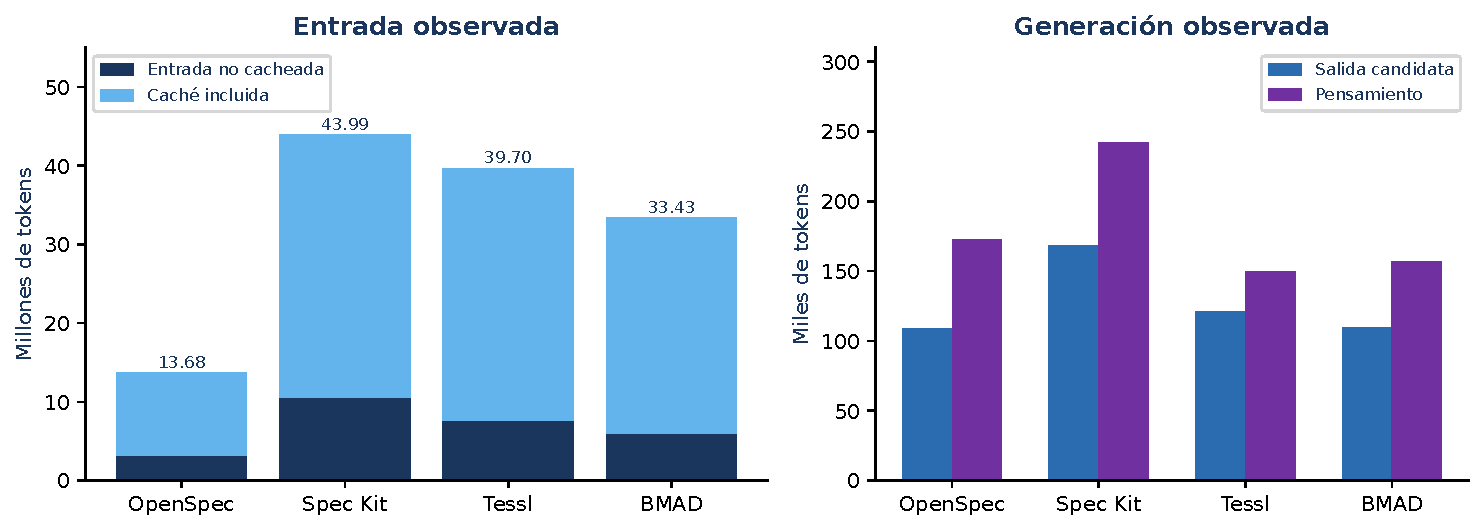
\includegraphics[width=.98\textwidth]{tetris-etapa2-assets/consumo.pdf}
\caption{Entrada y generación observadas. Las dos escalas son distintas; la caché forma parte de la entrada. Kiro se omite porque sus tokens son N/D. Los vacíos de OpenSpec y Tessl impiden tratar las barras como consumo completo.}\label{fig:consumo_tetris_e2}\end{figure}

\begin{table}[H]\centering\small\setlength{\tabcolsep}{4pt}\renewcommand{\arraystretch}{1.06}
\caption{Intentos, duración instrumentada y solicitudes API conocidas}
\label{tab:esfuerzo_tetris_e2}
\begin{tabularx}{\textwidth}{l Y Y Y}\toprule

\textbf{Herramienta} & \textbf{Intentos / inicio de modelo} & \textbf{Segundos CLI} & \textbf{API: intentos / errores / éxitos} \\ \midrule

OpenSpec & 10 / 9; 01 N/D & 2.862,534 & 127 / 3 / 124 \\

Spec Kit & 17 / 16 & 11.526,593 & 645 / 121 / 524 \\

Tessl & 8 / 7; 02 N/D & 3.642,237 & 400 / 53 / 347 \\

BMAD & 7 / 7 & 3.563,083 & 242 / 13 / 229 \\

Kiro & 7 / 7 & 4.157,155 & N/D \\

\bottomrule\end{tabularx}

\par\smallskip\begin{minipage}{\textwidth}\footnotesize Duración desconocida: OpenSpec 01, Spec Kit 01/03 y Kiro 05. La suma incluye el fallo del lanzador Spec Kit 06 (0,084 s, sin inferencia). Los intentos API son parciales: faltan OpenSpec 01/02/05/06, Spec Kit 01/03/11/12, Tessl 02 y BMAD 04/05/06. Un exit 0 no prueba aceptación funcional.\end{minipage}

\end{table}

\begin{figure}[H]\centering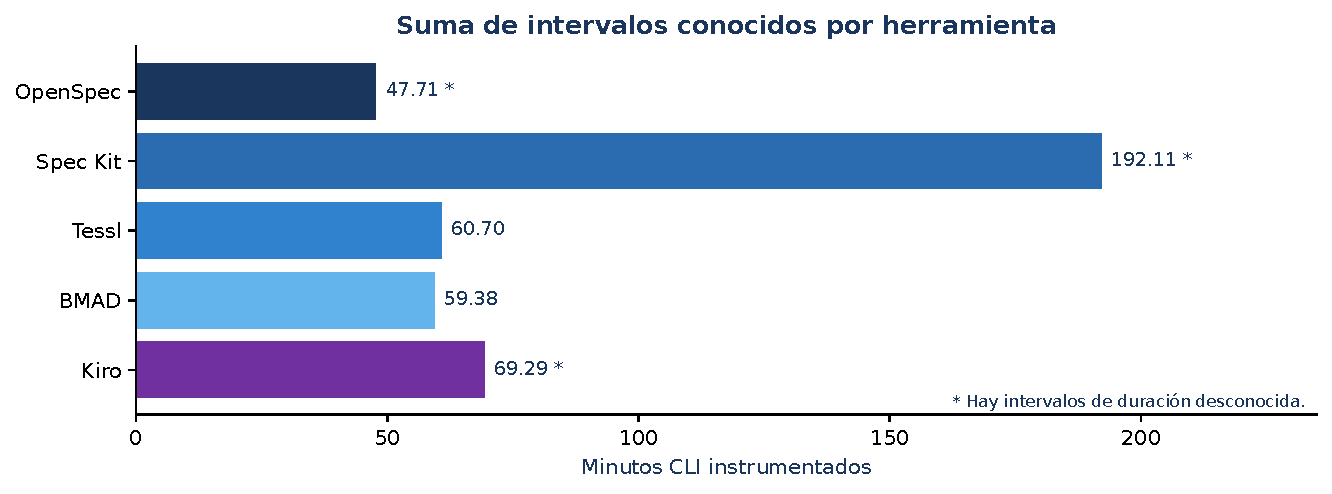
\includegraphics[width=.98\textwidth]{tetris-etapa2-assets/tiempos.pdf}
\caption{Tiempo CLI conocido. Excluye intervalos no instrumentados y trabajo externo; no representa tiempo humano ni duración calendario de cada etapa.}\label{fig:tiempos_tetris_e2}\end{figure}

En Kiro se recuperaron \textbf{101,369363 créditos} de 02/03/04/06/07; 01 y 05 permanecen N/D. Los valores por intento son 5,897180; 8,026105; 49,458271; 18,924292 y 19,063515, respectivamente. El tiempo de agente conocido es 3.997,507 s, con 01/05 desconocidos; es otra métrica y no se añade al tiempo CLI. Los IDs de solicitudes y el porcentaje de contexto no se convierten en tokens.

Para mantener la comparación con la etapa 1 se calcula únicamente un \textit{costo teórico normalizado}, usando los coeficientes de referencia ya adoptados en el capítulo:
\[
 C_{\mathrm{ref}}=\frac{1{,}5(I-C)+0{,}15C+9O}{10^6}.
\]
$I$ es entrada, $C$ caché incluida y $O$ salida candidata. Estos coeficientes no se presentan como tarifas vigentes ni facturación real. El cálculo excluye pensamiento, diferencias tarifarias entre modelos, descuentos y créditos; por tanto, no es un límite inferior garantizado de una factura. Para Kiro se conserva el escenario de 0,03 USD por crédito del capítulo, sólo sobre créditos conocidos.

\begin{table}[H]\centering\small\setlength{\tabcolsep}{4pt}\renewcommand{\arraystretch}{1.06}
\caption{Escenario de costo con los coeficientes de referencia del capítulo}
\label{tab:costo_tetris_e2}
\begin{tabularx}{\textwidth}{l Y Y}\toprule

\textbf{Herramienta} & \textbf{USD de referencia} & \textbf{Alcance} \\ \midrule

OpenSpec & 7,2697 & Contadores observados; omisiones indicadas en la tabla de tokens. \\

Spec Kit & 22,3879 & Contadores observados; omisiones indicadas en la tabla de tokens. \\

Tessl & 17,3040 & Contadores observados; omisiones indicadas en la tabla de tokens. \\

BMAD & 13,9943 & Contadores observados; omisiones indicadas en la tabla de tokens. \\

Kiro & 3,0411 & Escenario sobre créditos conocidos; 01/05 N/D. \\

\bottomrule\end{tabularx}

\end{table}

Las solicitudes API no se confunden con mensajes retenidos: OpenSpec conserva 229 respuestas documentadas (139 retenidas y 90 históricas); Spec Kit, 560 respuestas JSONL. Estos recuentos tienen otra cobertura y pueden omitir roles auxiliares. Los ciclos internos de lectura, edición, ejecución o escaneo tampoco se contabilizan como nuevos prompts externos. La trazabilidad por intento se incluye al final de este caso.

\begin{table}[H]\centering\small\setlength{\tabcolsep}{4pt}\renewcommand{\arraystretch}{1.06}
\caption{Llamados a herramientas observables dentro de las invocaciones}
\label{tab:llamados_tetris_e2}
\begin{tabularx}{\textwidth}{l Y Y}\toprule

\textbf{Herramienta} & \textbf{Llamados conocidos} & \textbf{Cobertura del contador} \\ \midrule

OpenSpec & 127 & Estadísticas completas de 03/04/07/08/09/10; otros cuatro intentos N/D. \\

Spec Kit & 520 & Doce salidas con estadísticas; 06 sin inferencia y cero llamados. 01/03/11/12 N/D. \\

Tessl & 351 & Siete salidas con estadísticas; 02 N/D. \\

BMAD & 225 & Estadísticas de 01/02/03/07; 04/05/06 N/D. \\

Kiro & 416 & Eventos tool\_call de siete tramos retenidos; 05 no tiene cierre nativo. \\

\bottomrule\end{tabularx}

\par\smallskip\begin{minipage}{\textwidth}\footnotesize Son sumas observadas y parciales cuando se indica. La definición del CLI y los eventos ACP de Kiro no son idénticos. Incluyen lecturas y otras acciones, no sólo ediciones; éxito del wrapper no demuestra que una prueba o comando subyacente haya aprobado.\end{minipage}

\end{table}

\subsubsection{Dimensión B: Impacto en la Calidad del Código}

Se analizaron las fuentes finales con las coberturas verificadas y un período de código nuevo frente a la línea base propia. El gate experimental exige cobertura nueva de al menos 80\%, duplicación nueva no mayor que 3\% y cero incidencias nuevas. Es un gate configurado para el estudio; su aprobación no significa ausencia de hallazgos heredados ni equivalencia con todas las recomendaciones del producto. El campo \texttt{caycStatus} es distinto del estado del gate: en Tessl, BMAD y Kiro figura \texttt{non-compliant} en el JSON retenido aunque las tres condiciones experimentales se aprueban. No se oculta esa distinción.

\begin{table}[H]\centering\small\setlength{\tabcolsep}{4pt}\renewcommand{\arraystretch}{1.06}
\caption{Métricas estáticas finales de SonarQube}
\label{tab:sonar_tetris_e2}
\begin{tabularx}{\textwidth}{Y r r r r r}\toprule

\textbf{Métrica} & \textbf{OpenSpec} & \textbf{Spec Kit} & \textbf{Tessl} & \textbf{BMAD} & \textbf{Kiro} \\ \midrule

ncloc & 1.327 & 1.098 & 1.125 & 1.039 & 784 \\

Líneas Sonar & 1.599 & 1.355 & 1.398 & 1.222 & 1.292 \\

Bugs & 0 & 0 & 0 & 0 & 0 \\

Vulnerabilidades & 0 & 0 & 1 & 1 & 0 \\

Code smells & 0 & 0 & 9 & 12 & 7 \\

Security hotspots & 0 & 0 & 0 & 0 & 0 \\

Deuda (min) & 0 & 0 & 46 & 81 & 23 \\

Complejidad ciclomática & 138 & 194 & 148 & 148 & 153 \\

Complejidad cognitiva & 111 & 148 & 120 & 157 & 114 \\

Duplicación global (\%) & 0,0 & 0,0 & 0,0 & 2,8 & 0,0 \\

Cobertura global (\%) & 90,3 & 83,9 & 86,9 & 89,6 & 93,2 \\

Seguridad / fiabilidad / mantenibilidad & A / A / A & A / A / A & C / A / A & C / A / A & A / A / A \\

Gate final & OK & OK & OK & OK & OK \\

\bottomrule\end{tabularx}

\end{table}

\begin{table}[H]\centering\small\setlength{\tabcolsep}{4pt}\renewcommand{\arraystretch}{1.06}
\caption{Condiciones efectivamente evaluadas sobre código nuevo}
\label{tab:gate_tetris_e2}
\begin{tabularx}{\textwidth}{l Y Y Y}\toprule

\textbf{Herramienta} & \textbf{Cobertura nueva (\%)} & \textbf{Duplicación nueva (\%)} & \textbf{Incidencias nuevas} \\ \midrule

OpenSpec & 83,0 & 0,0 & 0 \\

Spec Kit & 86,6 & 0,0 & 0 \\

Tessl & 82,7 & 0,0 & 0 \\

BMAD & 85,8 & 2,47855 & 0 \\

Kiro & 88,7 & 0,0 & 0 \\

\bottomrule\end{tabularx}

\par\smallskip\begin{minipage}{\textwidth}\footnotesize Umbrales: cobertura $\geq80\%$, duplicación $\leq3\%$ e incidencias $=0$. La duplicación global de BMAD (2,8\%) y la nueva (2,47855\%) tienen denominadores distintos. Un gate inicial OK con cero condiciones evaluadas no acredita estas condiciones finales.\end{minipage}

\end{table}

\begin{figure}[H]\centering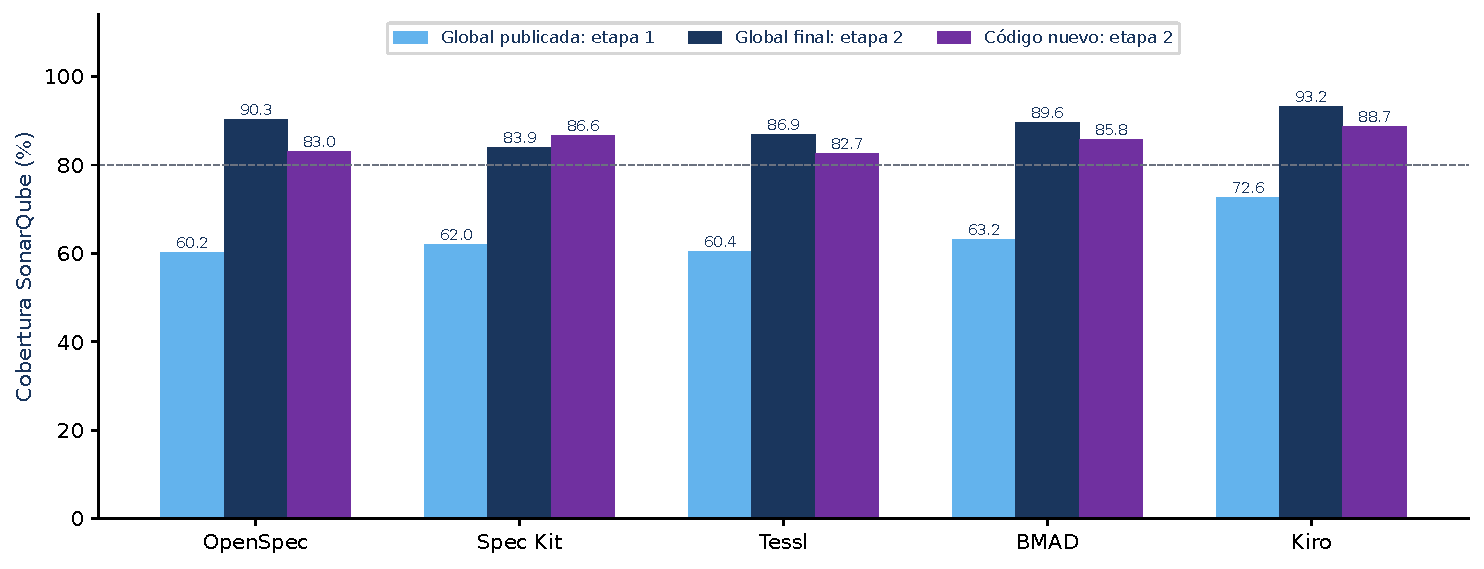
\includegraphics[width=.98\textwidth]{tetris-etapa2-assets/cobertura.pdf}
\caption{Cobertura global publicada en la etapa 1, global final de la etapa 2 y cobertura de código nuevo. La línea de 80\% corresponde sólo al umbral de código nuevo. Los tres indicadores no comparten el mismo denominador.}\label{fig:cobertura_tetris_e2}\end{figure}

\begin{figure}[H]\centering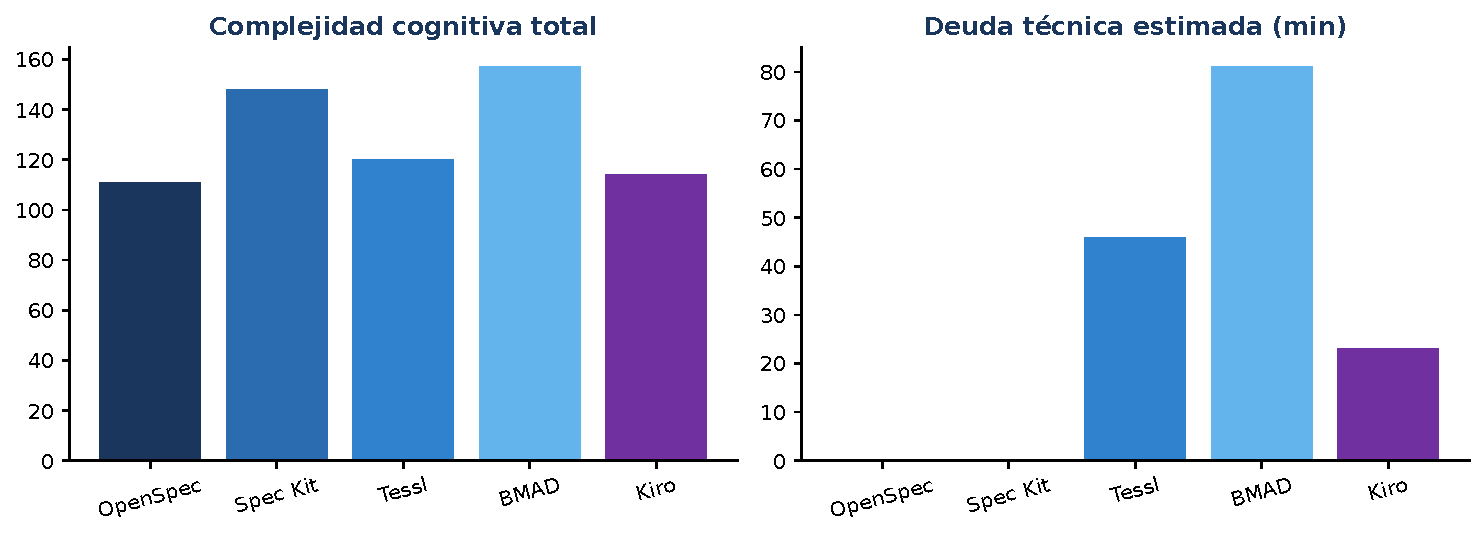
\includegraphics[width=.98\textwidth]{tetris-etapa2-assets/mantenibilidad.pdf}
\caption{Complejidad cognitiva y deuda técnica final. Son cantidades absolutas sobre fuentes de tamaño distinto; no constituyen un índice compuesto de calidad ni una medida de escalabilidad.}\label{fig:mantenibilidad_tetris_e2}\end{figure}

OpenSpec y Spec Kit terminaron sin bugs, vulnerabilidades ni olores reportados. Tessl conserva una vulnerabilidad heredada y nueve olores; BMAD conserva una vulnerabilidad heredada y doce olores; Kiro conserva siete olores. La observación del PRNG heredado se mantuvo cuando correspondía, sin desactivar la regla para mejorar artificialmente el resultado. Cero incidencias nuevas no equivale a cero incidencias totales.

Respecto a la tabla publicada de la etapa 1, los hallazgos finales (bugs + vulnerabilidades + olores) pasan de 16 a 0 en OpenSpec; de 9 a 0 en Spec Kit; de 14 a 10 en Tessl; de 14 a 13 en BMAD y de 10 a 7 en Kiro. La densidad final es 0,00; 0,00; 8,89; 12,51 y 8,93 hallazgos/KLOC, usando exclusivamente ncloc de Sonar. Esta evolución es descriptiva: las líneas base específicas reanalizadas al inicio de la etapa 2 no reproducen necesariamente todos los contadores publicados antes. Por ejemplo, Tessl registra 14 olores/72 min y Kiro 7 olores/23 min en su nueva base, frente a 13/71 y 10/38 en la tabla anterior. Se conserva la diferencia sin atribuirla a una causa no acreditada.

En BMAD, el primer cierre de 07 reutilizó un XML de cobertura anterior a la extracción de un helper: describía 177 sentencias en vez de 179. El investigador conservó ese resultado, regeneró XML/LCOV sobre la fuente congelada y repitió Sonar sin modificar el código. Las cifras aquí publicadas corresponden al análisis final \path{0b7d51b5-586c-4af2-8c0f-221a07a197d3}, no al cierre previo. Esta corrección es de evidencia, no una nueva implementación del modelo.

\subsubsection{Dimensión C: Evolución de la Especificación}

Se cuentan líneas físicas y caracteres Unicode del texto UTF-8, con BOM retirado y saltos de línea normalizados. El código incluye pruebas y excluye dependencias, builds, cobertura generada, lockfiles y documentación. Por eso sus líneas físicas no son ncloc. El corpus de especificación compara Markdown nativo nuevo de la etapa 2: excluye copias de la etapa 1, transcritos, bitácoras del investigador y archivos duplicados/archivados. Se distingue volumen de documentación de completitud o calidad semántica.

\begin{table}[H]\centering\small\setlength{\tabcolsep}{4pt}\renewcommand{\arraystretch}{1.06}
\caption{Inventario homogéneo de código y pruebas antes y después de la ampliación}
\label{tab:codigo_tetris_e2}
\begin{tabularx}{\textwidth}{l Y Y Y Y}\toprule

\textbf{Herramienta} & \textbf{Archivos base / final} & \textbf{Líneas base / final} & \textbf{Caracteres base / final} & \textbf{Delta líneas} \\ \midrule

OpenSpec & 13 / 15 & 1.366 / 2.238 & 39.957 / 69.725 & 872 \\

Spec Kit & 27 / 29 & 1.412 / 3.972 & 41.297 / 122.186 & 2.560 \\

Tessl & 19 / 22 & 1.299 / 2.829 & 37.962 / 86.150 & 1.530 \\

BMAD & 9 / 12 & 1.036 / 2.040 & 31.549 / 61.593 & 1.004 \\

Kiro & 23 / 37 & 1.207 / 3.691 & 33.641 / 119.547 & 2.484 \\

\bottomrule\end{tabularx}

\end{table}

\begin{table}[H]\centering\small\setlength{\tabcolsep}{4pt}\renewcommand{\arraystretch}{1.06}
\caption{Corpus de Markdown nativo nuevo de la etapa 2}
\label{tab:specs_tetris_e2}
\begin{tabular*}{\textwidth}{@{\extracolsep{\fill}}l r r r r r}\toprule

\textbf{Herramienta} & \textbf{Archivos} & \textbf{Líneas} & \textbf{Caracteres} & \textbf{Líneas/archivo} & \textbf{ncloc/línea spec} \\ \midrule

OpenSpec & 4 & 262 & 20.582 & 65,50 & 5,06 \\

Spec Kit & 8 & 1.337 & 89.432 & 167,12 & 0,82 \\

Tessl & 2 & 343 & 35.281 & 171,50 & 3,28 \\

BMAD & 8 & 977 & 78.537 & 122,12 & 1,06 \\

Kiro & 3 & 886 & 92.802 & 295,33 & 0,88 \\

\bottomrule\end{tabular*}

\par\smallskip\begin{minipage}{\textwidth}\footnotesize En Spec Kit, el inventario original incluye además OpenAPI JSON: 9 archivos, 1.713 líneas y 99.987 caracteres. Al retirar ese JSON de 376 líneas y 10.555 caracteres quedan los 8 Markdown de esta tabla. La etapa 1 publicada también usó 8 Markdown/1.002 líneas. No se mezclan ambos denominadores.\end{minipage}

\end{table}

\begin{figure}[H]\centering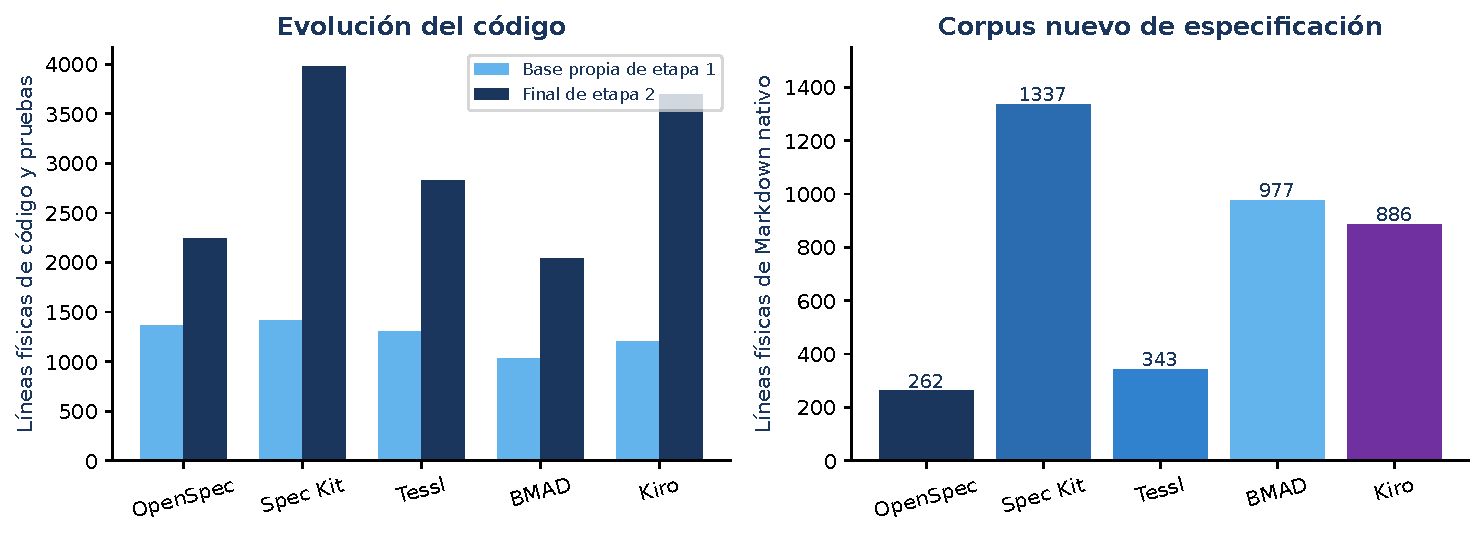
\includegraphics[width=.98\textwidth]{tetris-etapa2-assets/artefactos.pdf}
\caption{Crecimiento del código y volumen de especificación nueva. Los paneles emplean corpus distintos y declarados; una especificación más larga no demuestra mejor implementación.}\label{fig:artefactos_tetris_e2}\end{figure}

Los artefactos nativos conservan las estructuras de cada herramienta. OpenSpec aporta propuesta, diseño, tareas y spec de cambio: 14 requisitos nuevos y uno modificado. Spec Kit aporta ocho Markdown de requisitos, checklist, contrato, modelo de datos, investigación, plan, guía rápida y tareas, además del contrato OpenAPI JSON separado. Tessl conserva \texttt{requirements.md} y \texttt{session\_notes.md}; este segundo documento mezcla decisiones y notas, y mantiene un párrafo antiguo de ERROR aun después del cierre. BMAD aporta ocho Markdown principales de PRD, arquitectura, épicas, especificación e historias; los 24 IDs funcionales nuevos declarados no se equiparan automáticamente a 24 requisitos atómicos. Kiro mantiene requisitos, diseño y tareas.

El volumen nuevo de la etapa 2 se informa separado del corpus heredado de la etapa 1: 4/442, 8/1.002, 2/136, 6/1.120 y 3/608 archivos/líneas para OpenSpec, Spec Kit, Tessl, BMAD y Kiro, respectivamente. En BMAD se conservaron los seis documentos heredados sin cambios. Las densidades de código final son 149,20; 136,97; 128,59; 170,00 y 99,76 líneas/archivo. El cociente ncloc/líneas de spec es sólo una relación entre dos inventarios; no mide precisión, fidelidad ni mantenimiento.

Se prepararon corpus para un eventual análisis de tópicos, pero no se entrenó BERTopic en este cierre. No se presentan tópicos, similitudes BERT, puntuaciones semánticas ni métricas de escalabilidad que no hayan sido efectivamente medidas. El estado de tareas del workflow no sustituye evidencia de ejecución: en BMAD, las cuatro retrospectivas opcionales marcadas en YAML no tienen artefactos verificados y no se cuentan como realizadas; un campo \texttt{last\_updated} atrasado tampoco se usa como cronómetro.

\subsubsection{Dimensión D: Validación Funcional}

El catálogo común contiene 20 criterios S2-01--S2-20 y todos quedaron respaldados por evidencia final en las cinco herramientas. Se separan 18 criterios generales de dos reglas de puntuación comprobadas en estados de dominio preparados (tres y cuatro filas); estas últimas no se presentan como jugadas ordinarias alcanzadas por un usuario en la variante sin rotación. Tampoco se interpreta 20/20 como veinte pruebas de API ni como una tasa de aceptación de veinte partidas de navegador. Cada criterio se apoya en el mecanismo apropiado: HTTP, dominio, contrato, React, observación de navegador o compilación.

\begin{table}[H]\centering\small\setlength{\tabcolsep}{4pt}\renewcommand{\arraystretch}{1.06}
\caption{Mapa del catálogo común y mecanismos de validación}
\label{tab:catalogo_tetris_e2}
\begin{tabularx}{\textwidth}{l Y Y}\toprule

\textbf{IDs S2} & \textbf{Comportamiento} & \textbf{Mecanismo} \\ \midrule

01 & Creación: contadores iniciales, Hold vacío y vista previa válida & HTTP y dominio \\

02 & Dos lecturas sin mutación ni consumo aleatorio & HTTP y dominio \\

03 & Fijación sin filas: cero puntos y avance correcto de pieza & HTTP y dominio \\

04--05 & Una/dos filas: 100/300 por nivel previo & Dominio controlado \\

06--07 & Tres/cuatro filas: 500/800 por nivel previo & Reglas aisladas; no juego ordinario \\

08--09 & Cruce 9 a 10 líneas y gravedad mínima de 100 ms & Dominio y fixture de transición \\

10--12 & Primer Hold, rechazo del segundo y desbloqueo/intercambio posterior & HTTP y dominio \\

13--14 & Aparición bloqueada y estado terminal inmutable & Dominio; navegador para evidencia visual \\

15--16 & Reinicio, rutas compatibles, nuevo Hold y error 404 & HTTP y contrato \\

17 & HUD, Next, Hold, tecla C y disponibilidad del botón & React y observación de navegador \\

18 & Intervalo autoritativo, cola y respuestas antiguas & React con tiempo/respuestas controlados \\

19 & Grilla, movimiento, colisión, fijación, borrado y fin de etapa 1 & Pruebas de regresión \\

20 & Build de producción desde dependencias registradas & Compilación \\

\bottomrule\end{tabularx}

\end{table}

\begin{table}[H]\centering\small\setlength{\tabcolsep}{4pt}\renewcommand{\arraystretch}{1.06}
\caption{Pruebas finales y verificaciones complementarias}
\label{tab:pruebas_tetris_e2}
\begin{tabularx}{\textwidth}{l Y Y}\toprule

\textbf{Herramienta} & \textbf{Backend / frontend propios} & \textbf{Controles externos o complementarios} \\ \midrule

OpenSpec & 20 / 5 & HTTP 7/7; dominio y React acreditan los demás IDs; build y lint aprobados. \\

Spec Kit & 35 / 38 & HTTP 7 registros para 8 IDs; contrato 9/9; casos de cola/temporizador y dominio controlado. \\

Tessl & 23 / 17 & Dominio 17/17; HTTP 7/7; contrato 9/9; concurrencia 6/6 y un caso adicional 1/1. \\

BMAD & 18 / 14 & Dominio externo 24/24 y frontend externo 11/11; regresiones originales preservadas. \\

Kiro & 120 / 49 & Dominio 15; HTTP 7; contrato 9; concurrencia 5; 38 regresiones originales aprobadas y una xfail declarada. \\

\bottomrule\end{tabularx}

\par\smallskip\begin{minipage}{\textwidth}\footnotesize Los tamaños de suite y las versiones de los frameworks difieren; no se suman estos recuentos para construir un ranking. Los tests propios no son la misma unidad que los criterios comunes o los controles independientes.\end{minipage}

\end{table}

\begin{table}[H]\centering\small\setlength{\tabcolsep}{4pt}\renewcommand{\arraystretch}{1.06}
\caption{Coberturas complementarias con el denominador declarado}
\label{tab:coberturas_tests_tetris_e2}
\begin{tabularx}{\textwidth}{l Y Y}\toprule

\textbf{Herramienta} & \textbf{Backend} & \textbf{Frontend} \\ \midrule

OpenSpec & 94\% sobre aplicación & 92,96\% de líneas \\

Spec Kit & 92\% sobre aplicación & 80,26\% sentencias; 70,25\% ramas; 97,14\% funciones; 84,07\% líneas \\

Tessl & 198/210 líneas: 94,29\% & LCOV: 143/160 líneas (89,38\%); 97/136 ramas (71,32\%); 29/30 funciones (96,67\%) \\

BMAD & 166/179 sentencias: 92,74\% & 89,71\% sentencias; 77,53\% ramas; 100\% funciones; 95,54\% líneas \\

Kiro & 245/247 sentencias: 99,19\% & 88,58\% sentencias; 77,55\% ramas; 92,68\% funciones; 94,47\% líneas \\

\bottomrule\end{tabularx}

\par\smallskip\begin{minipage}{\textwidth}\footnotesize No se convierten porcentajes de líneas o sentencias de pytest/Vitest en cobertura global de Sonar, que también considera condiciones. Los subtotales Tessl se calcularon del XML final y los acumulados LF/LH, BRF/BRH y FNF/FNH del LCOV preservado. Las diferencias de Vitest y de inclusión de archivos afectan los denominadores.\end{minipage}

\end{table}

En Kiro se mantuvo como \texttt{xfail} una igualdad cerrada del esquema original de respuesta, porque la ampliación agrega siete campos de forma intencionada; por tanto, no se afirma que las 39 pruebas originales pasan sin adaptación. En BMAD se conservaron 13 nombres de pruebas y 52 aserciones AST originales; los fixtures se adaptaron a la cola de acciones. Su prueba del elemento raíz es débil por sí sola: el arranque real se verificó además en navegador.

Las auditorías finales de dependencias JavaScript y los builds quedaron aprobados en los cierres documentados. BMAD verificó además el entorno Python completo: 50 paquetes, cero vulnerabilidades y cero omisiones. No se extrapola ese alcance de auditoría Python a las otras herramientas. Los fallos iniciales de pruebas, dependencias o Sonar se conservaron para reconstruir las correcciones; no fueron sustituidos por los resultados finales.

\paragraph{Evidencia visual de las implementaciones.}

Las capturas siguientes proceden de las evidencias conservadas de cada cierre. Se diferencia la aplicación en el navegador de los paneles derivados de JSON y logs. Un fixture de transición o fin de partida se etiqueta como tal; una captura fija no demuestra por sí sola serialización o descarte de respuestas, que se acreditan con pruebas controladas.

\begin{figure}[H]\centering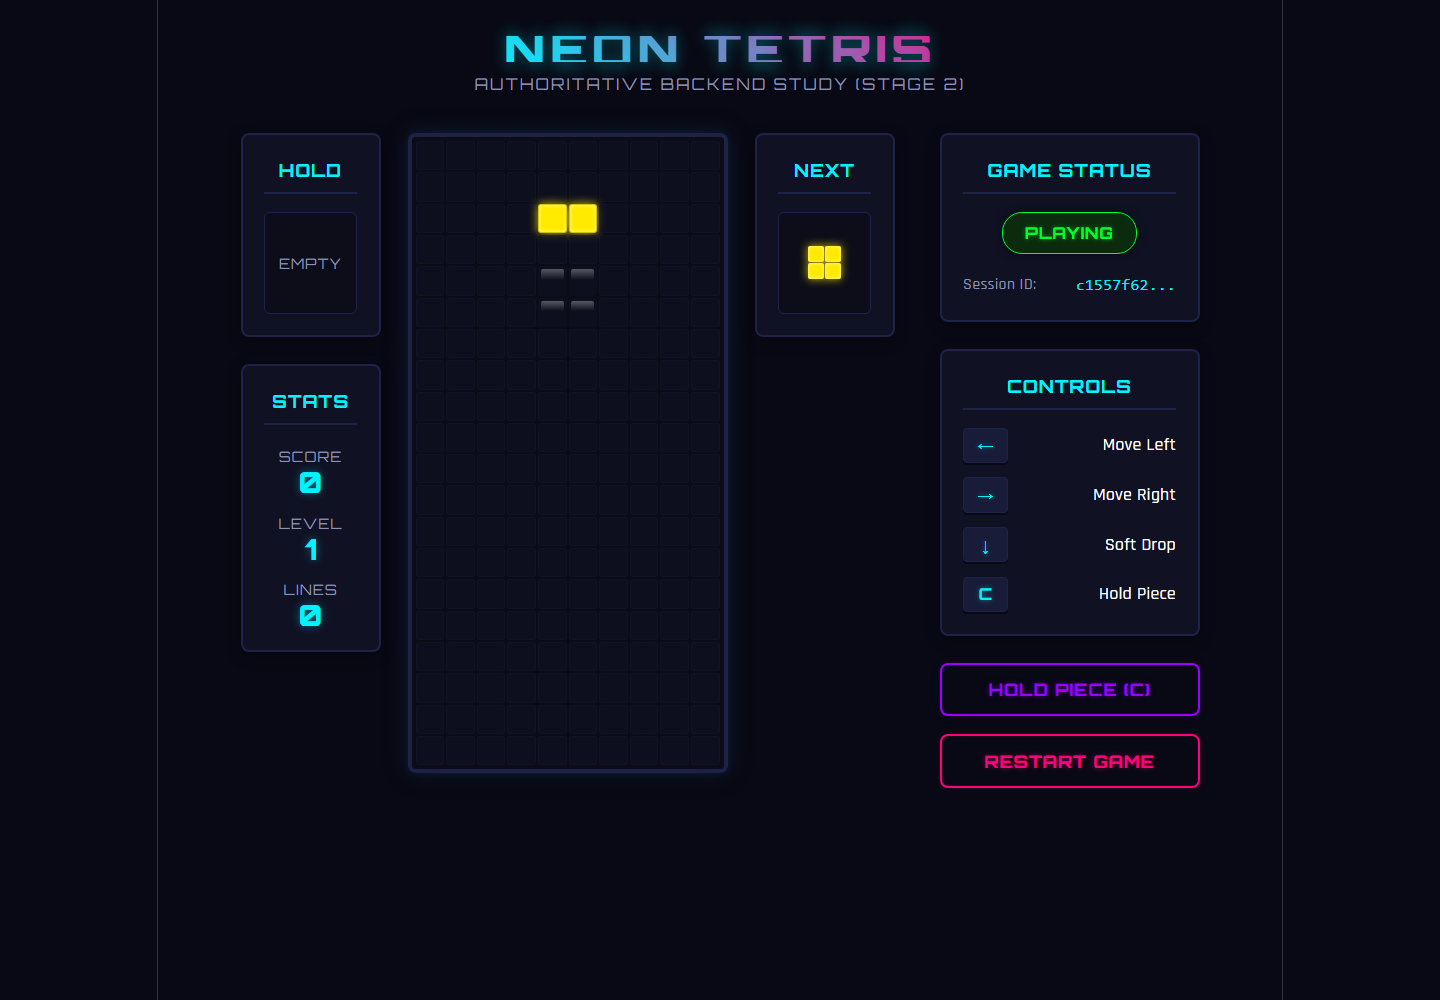
\includegraphics[width=.98\textwidth,height=.52\textheight,keepaspectratio]{tetris-etapa2-assets/openspec-ui.png}
\caption{OpenSpec: estado inicial, contadores, vista previa y controles de Hold. Captura de la aplicación; la ranura Hold todavía está vacía.}\label{fig:openspec-ui_tetris_e2}\end{figure}

\begin{figure}[H]\centering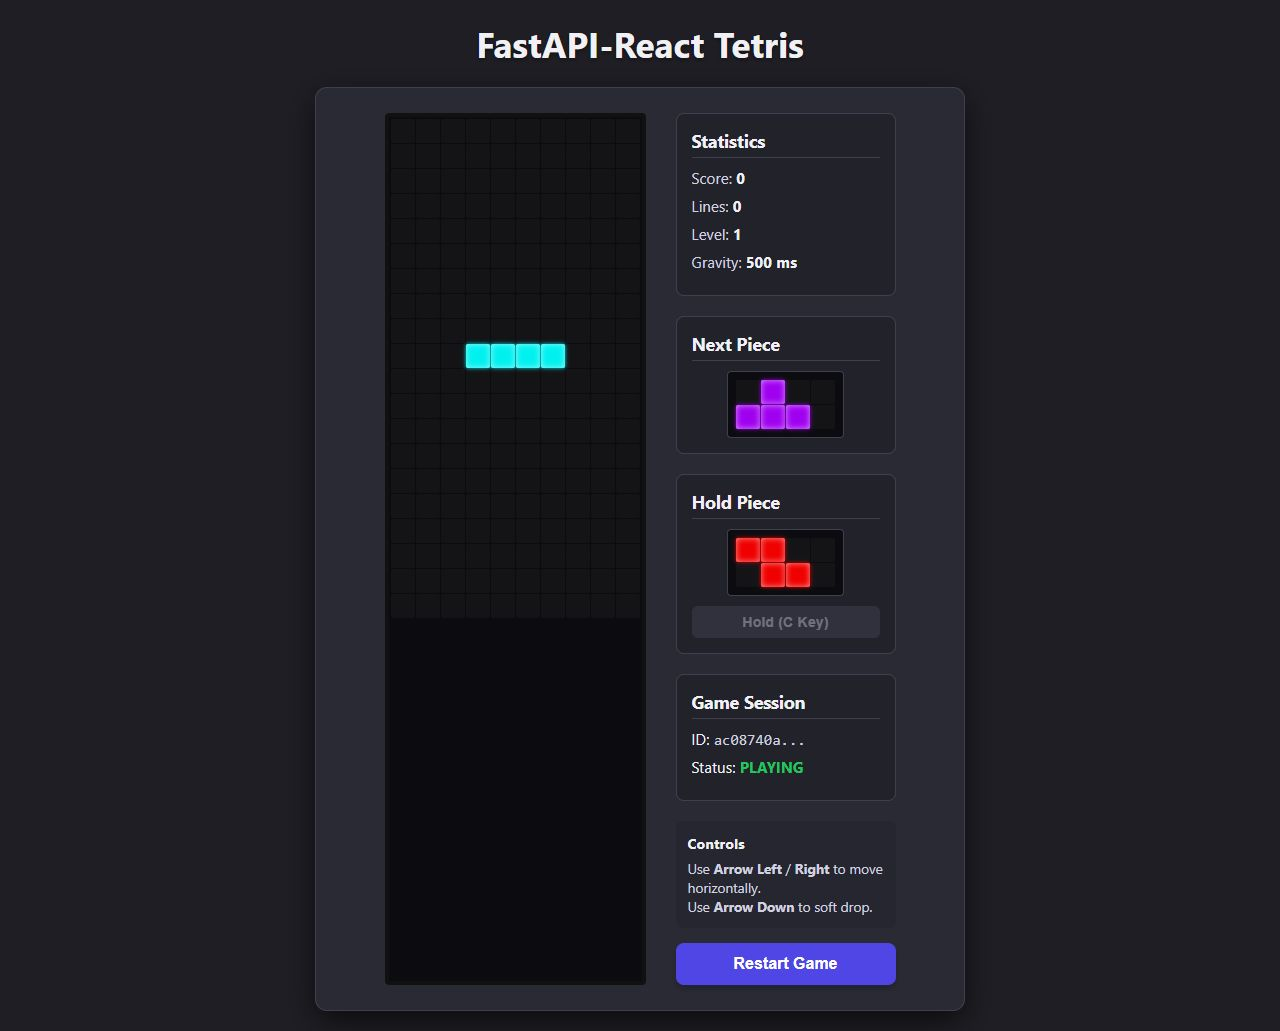
\includegraphics[width=.98\textwidth,height=.52\textheight,keepaspectratio]{tetris-etapa2-assets/speckit-ui.jpg}
\caption{Spec Kit: partida con pieza retenida y siguiente pieza visibles. Captura de la aplicación final.}\label{fig:speckit-ui_tetris_e2}\end{figure}

\begin{figure}[H]\centering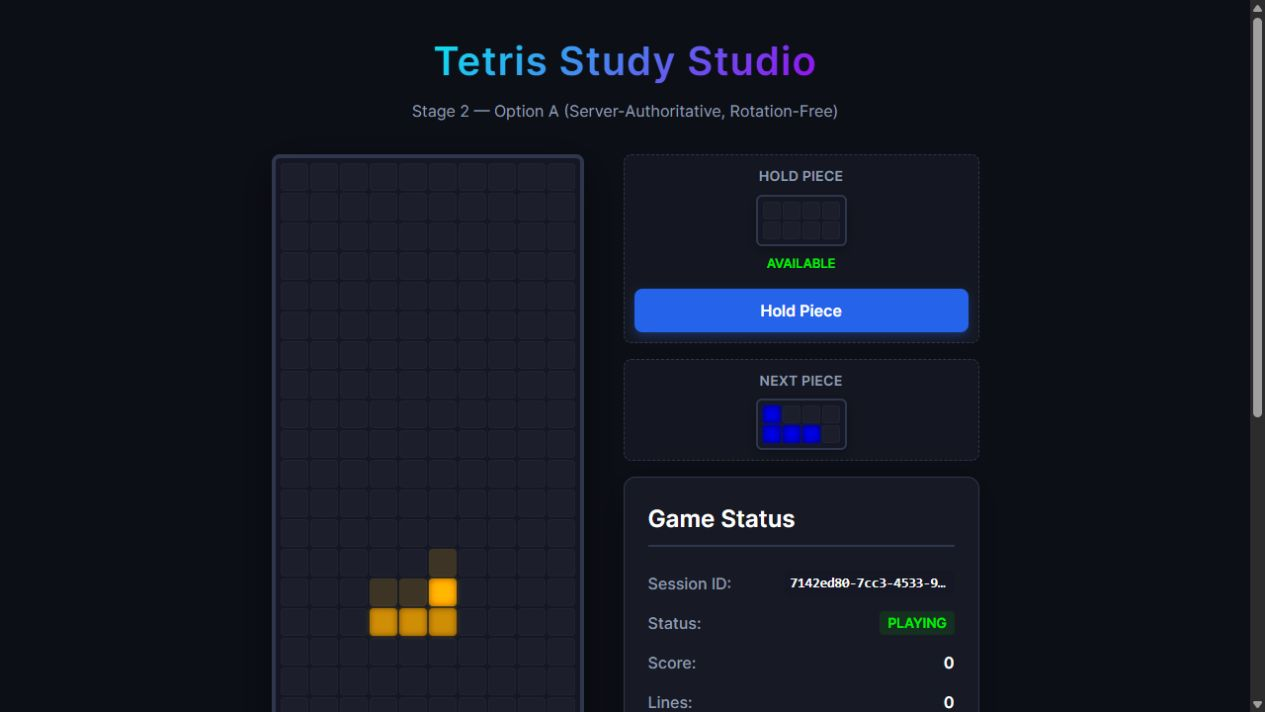
\includegraphics[width=.98\textwidth,height=.52\textheight,keepaspectratio]{tetris-etapa2-assets/tessl-ui.jpg}
\caption{Tessl: vista de la aplicación final. La evidencia se complementa con los controles y estados de las capturas siguientes.}\label{fig:tessl-ui_tetris_e2}\end{figure}

\begin{figure}[H]\centering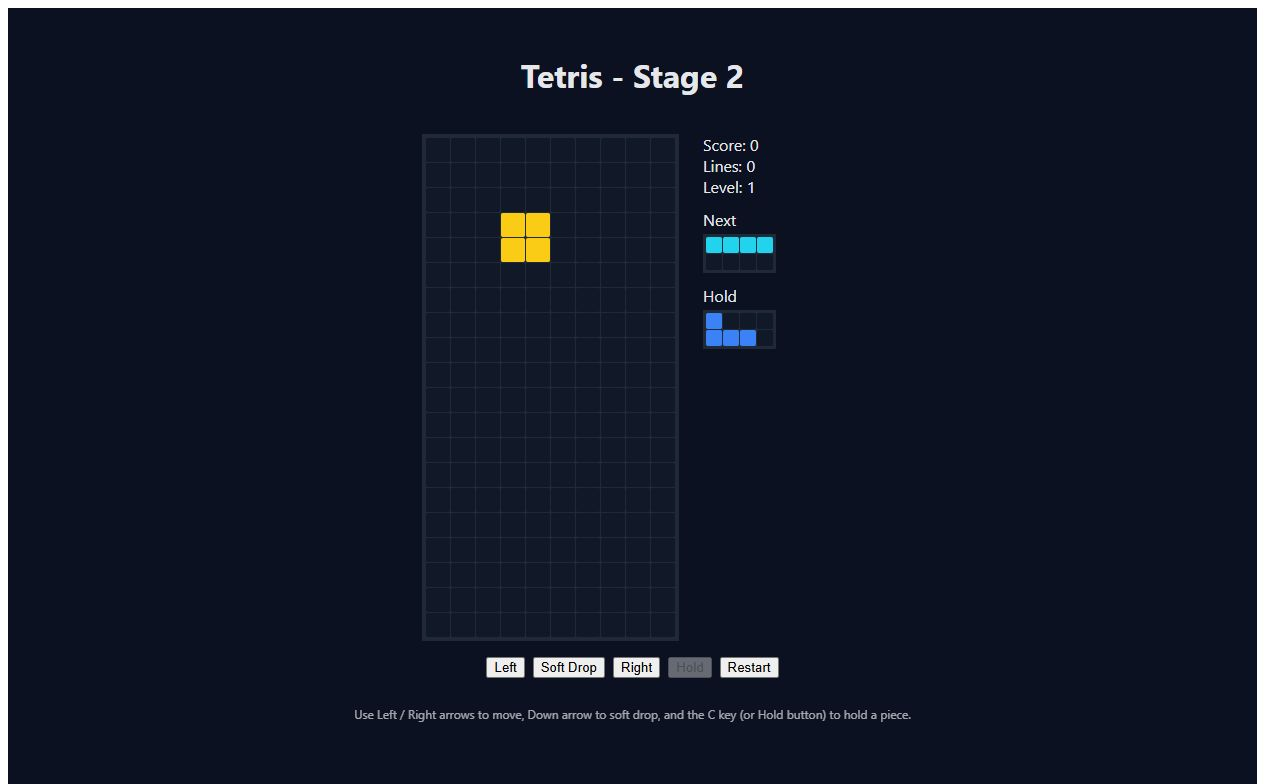
\includegraphics[width=.98\textwidth,height=.52\textheight,keepaspectratio]{tetris-etapa2-assets/kiro-ui.jpg}
\caption{Kiro: Hold ejecutado desde el botón, con pieza retenida y vista previa. Captura de la aplicación final.}\label{fig:kiro-ui_tetris_e2}\end{figure}

\begin{figure}[H]\centering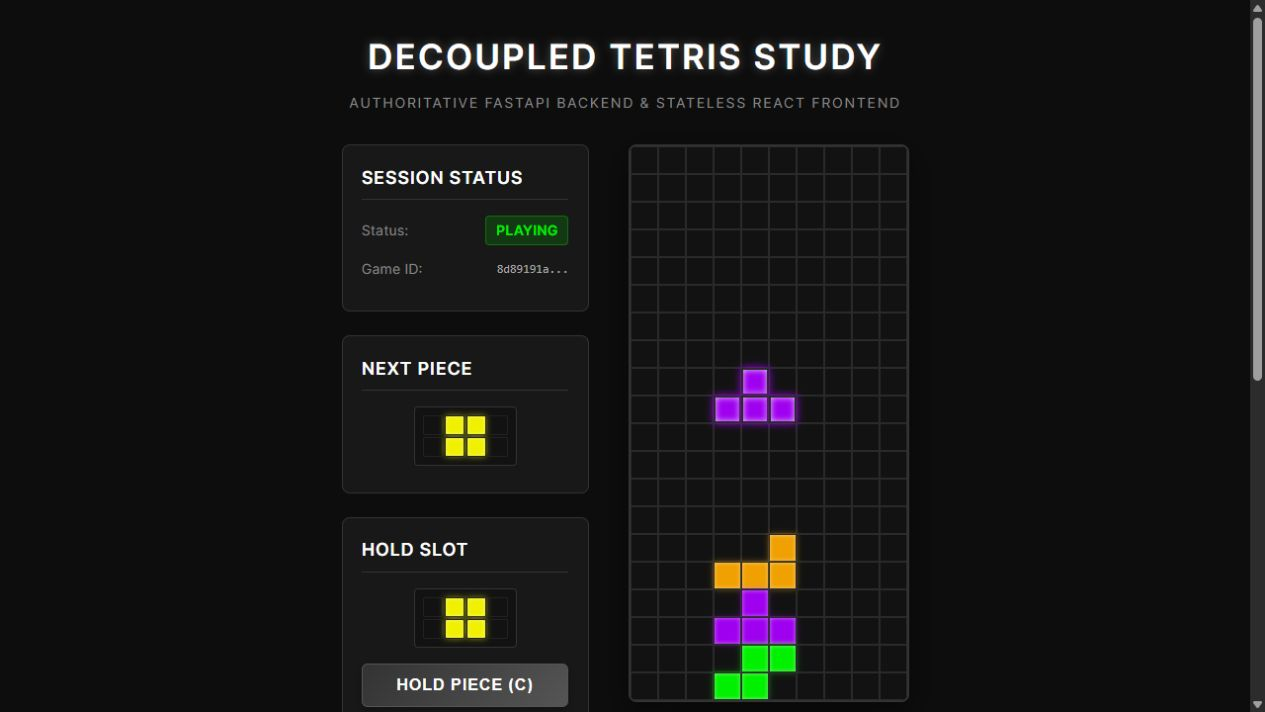
\includegraphics[width=.98\textwidth,height=.52\textheight,keepaspectratio]{tetris-etapa2-assets/bmad-ui.jpg}
\caption{BMAD: tablero, vista previa y ranura Hold ocupada. Captura del navegador; los contadores se observan al desplazar la misma página.}\label{fig:bmad-ui_tetris_e2}\end{figure}

\begin{figure}[H]\centering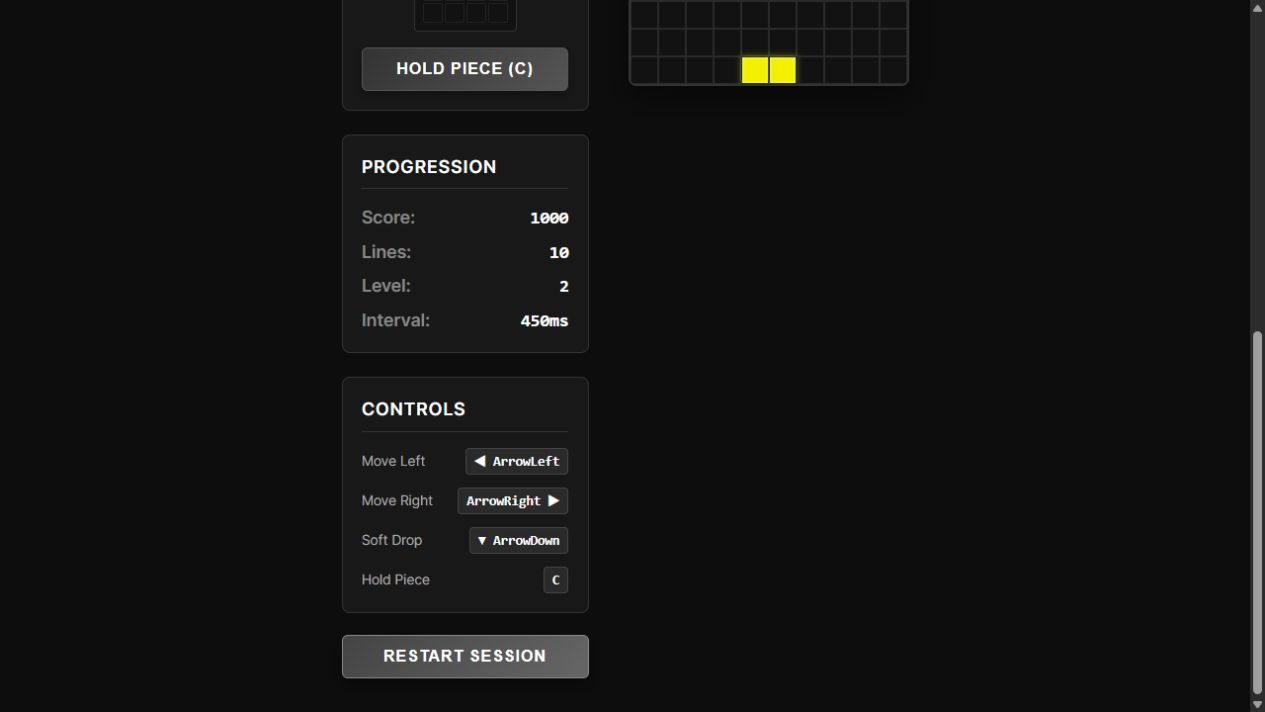
\includegraphics[width=.98\textwidth,height=.52\textheight,keepaspectratio]{tetris-etapa2-assets/bmad-level.jpg}
\caption{BMAD: fixture controlado de cruce de 9 a 10 líneas, 1.000 puntos, nivel 2 e intervalo de 450 ms. Es evidencia preparada de la transición, no una partida natural completa.}\label{fig:bmad-level_tetris_e2}\end{figure}

\begin{figure}[H]\centering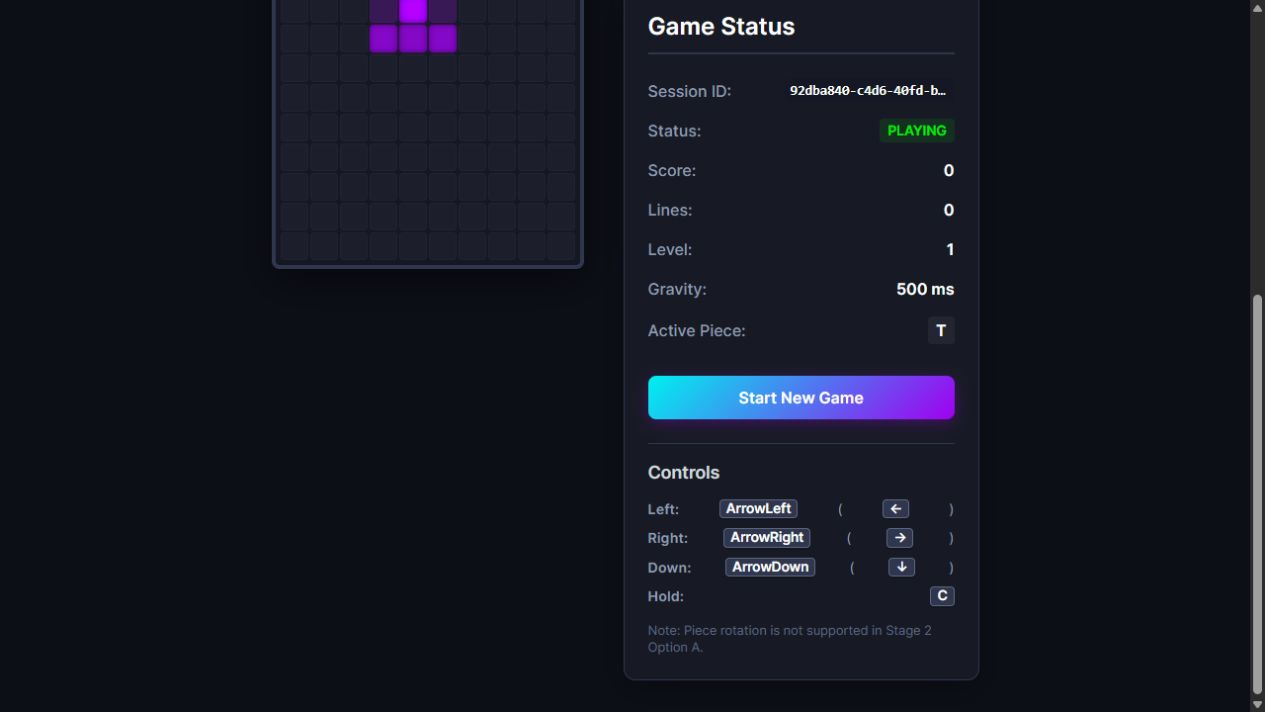
\includegraphics[width=.98\textwidth,height=.52\textheight,keepaspectratio]{tetris-etapa2-assets/tessl-hud.jpg}
\caption{Tessl: HUD autoritativo y botón/tecla de Hold. Es otro desplazamiento de la página, no una composición de pantallas.}\label{fig:tessl-hud_tetris_e2}\end{figure}

\begin{figure}[H]\centering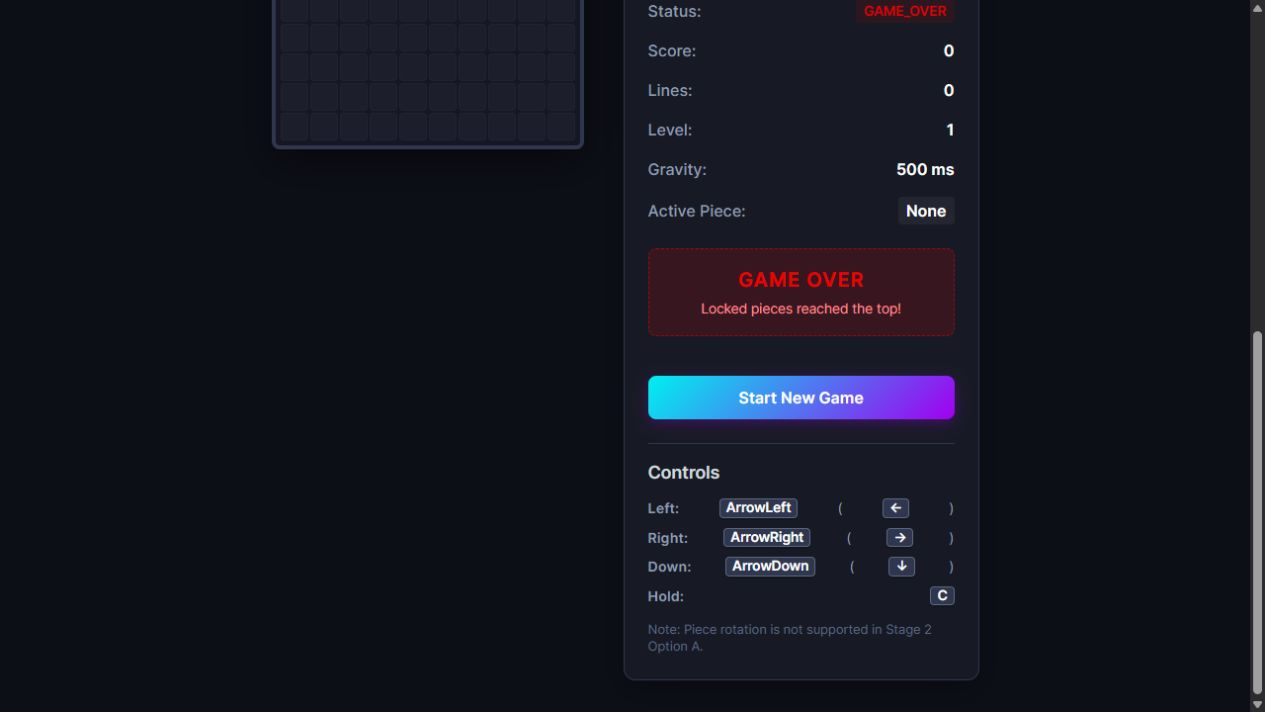
\includegraphics[width=.98\textwidth,height=.52\textheight,keepaspectratio]{tetris-etapa2-assets/tessl-terminal.jpg}
\caption{Tessl: fin de partida inducido por un fixture controlado; la pieza activa queda ausente y se conservan los contadores.}\label{fig:tessl-terminal_tetris_e2}\end{figure}

\subsubsection{Dimensión E: Intervención y Correcciones}

Se distinguen preguntas bloqueantes emitidas por el modelo, prompts externos de corrección, objetivos QA distintos, reintentos y remediación automática dentro de una invocación. La revisión de preguntas considera texto natural retenido dentro del intervalo de cada ejecución y evita duplicar mensajes por copias o reanudaciones. Un flujo sin interacción no justifica inferir cero preguntas. Estos recuentos no miden horas humanas ni la totalidad de las intervenciones de investigación.

\begin{table}[H]\centering\small\setlength{\tabcolsep}{4pt}\renewcommand{\arraystretch}{1.06}
\caption{Corrección externa y preguntas bloqueantes observadas}
\label{tab:intervencion_tetris_e2}
\begin{tabularx}{\textwidth}{l Y Y Y}\toprule

\textbf{Herramienta} & \textbf{Intentos QA / objetivos} & \textbf{Preguntas bloqueantes} & \textbf{Lectura del registro} \\ \midrule

OpenSpec & 10: remediación final; sin clasificación homologada & N/D & Incluye intervención manual de código posterior; se explica separadamente. \\

Spec Kit & 9 / 4 & 0 observadas & 21 mensajes naturales únicos revisados; incluye intentos fallidos y reintentos. \\

Tessl & 3 / 2 & 0 observadas & 132 mensajes revisados en los intervalos cerrados retenidos. \\

BMAD & 3 / 1 & 0 observadas & 145 mensajes revisados; 05/06/07 comparten el mismo objetivo. \\

Kiro & 3 / 2 & 1 observada & 05 pidió confirmación de alcance; se resolvió con autorización previa, sin una nueva respuesta humana. \\

\bottomrule\end{tabularx}

\par\smallskip\begin{minipage}{\textwidth}\footnotesize En OpenSpec no existe una auditoría de preguntas equivalente a las otras cuatro. Un cero observado es limitado a los mensajes retenidos y revisados; no demuestra inexistencia absoluta de preguntas no registradas. El texto de OpenSpec 10 identifica una invocación, no diez objetivos QA.\end{minipage}

\end{table}

\begin{itemize}
\item \textbf{OpenSpec.} 01 se interrumpió por red; 02 produjo texto sin archivos; 05 se interrumpió sin cambios y 06 quedó en Plan Mode sin escrituras. Tras la remediación 10, el investigador reemplazó dos literales repetidos de \texttt{backend/main.py} para cerrar S1192 y agregó pruebas/configuración de cobertura. Ese cambio manual de código se aparta de la regla de efectuar toda corrección mediante aclaración a la herramienta. El resultado final es de OpenSpec/Gemini con QA del investigador, no salida íntegramente automática. También se preservaron ajustes de especificación/tareas y sus responsables.
\item \textbf{Spec Kit.} 01 recibió argumentos vacíos por serialización del comando; 03 se interrumpió y 06 falló antes de inferencia. Los reintentos 11--16 no representan seis problemas independientes: pertenecen al mismo objetivo de cola/temporizador. En 13, un registro sintético precedió al prompt real completo; éste aparece antes de la primera respuesta con tokens y el intento no produjo cambios de aplicación. Los fallos y el acceso contextual quedaron en la auditoría de entrada.
\item \textbf{Tessl.} 02 recibió \texttt{BILLING\_DISABLED}; sus contadores no se imputan. Se utilizó el flujo real de contexto MCP/plugins locales, sin atribuirle un generador SDD remoto no usado. Se documentan correcciones internas en 05/07 sin revisión previa de spec: el hecho de haber escrito primero una especificación no prueba cumplimiento de ese orden en todas las correcciones. Las notas antiguas de ERROR y resúmenes de tiempos redactados por el modelo no sustituyen los registros instrumentados finales.
\item \textbf{BMAD.} El límite de 80 turnos produjo exit 53 en 04/05/06; 07 cerró las correcciones. 02 terminó con exit 0 pero con errores 429 y planificación incompleta. La revisión secuencial fue una adaptación explícita del workflow; no se afirma independencia entre revisores. La primera prueba externa de concurrencia aprobó 5/11: un \texttt{finally} antiguo de Hold alteraba la cola de una nueva generación. La corrección se canalizó por el flujo nativo y la repetición final aprobó 11/11. Las incidencias nuevas de Sonar pasaron por 31, 6 y 0; se mantuvieron las reglas y el gate. La corrección posterior del XML de cobertura se registra como ajuste de evidencia.
\item \textbf{Kiro.} 01 se interrumpió por cambio de cuenta; 02 ejecutó Vibe pese al flag solicitado y 03 revisó la spec nativa. La duración, el cierre y los créditos de 05 son desconocidos: un límite superior de observación no se transforma en tiempo facturado. En 04 hubo correcciones estilísticas sin revisión previa de specs, una desviación del procedimiento; en 07 sí se revisaron los tres artefactos antes del código. Auto no permite asegurar el modelo de backend ni su consumo por rol.
\end{itemize}

\paragraph{Paneles de calidad y consumo conservados.}

Los siguientes paneles reproducen datos conservados de los registros y se identifican explícitamente como vistas del investigador. Las tablas anteriores permiten contrastar sus valores sin depender de la legibilidad de la captura.

\begin{figure}[H]\centering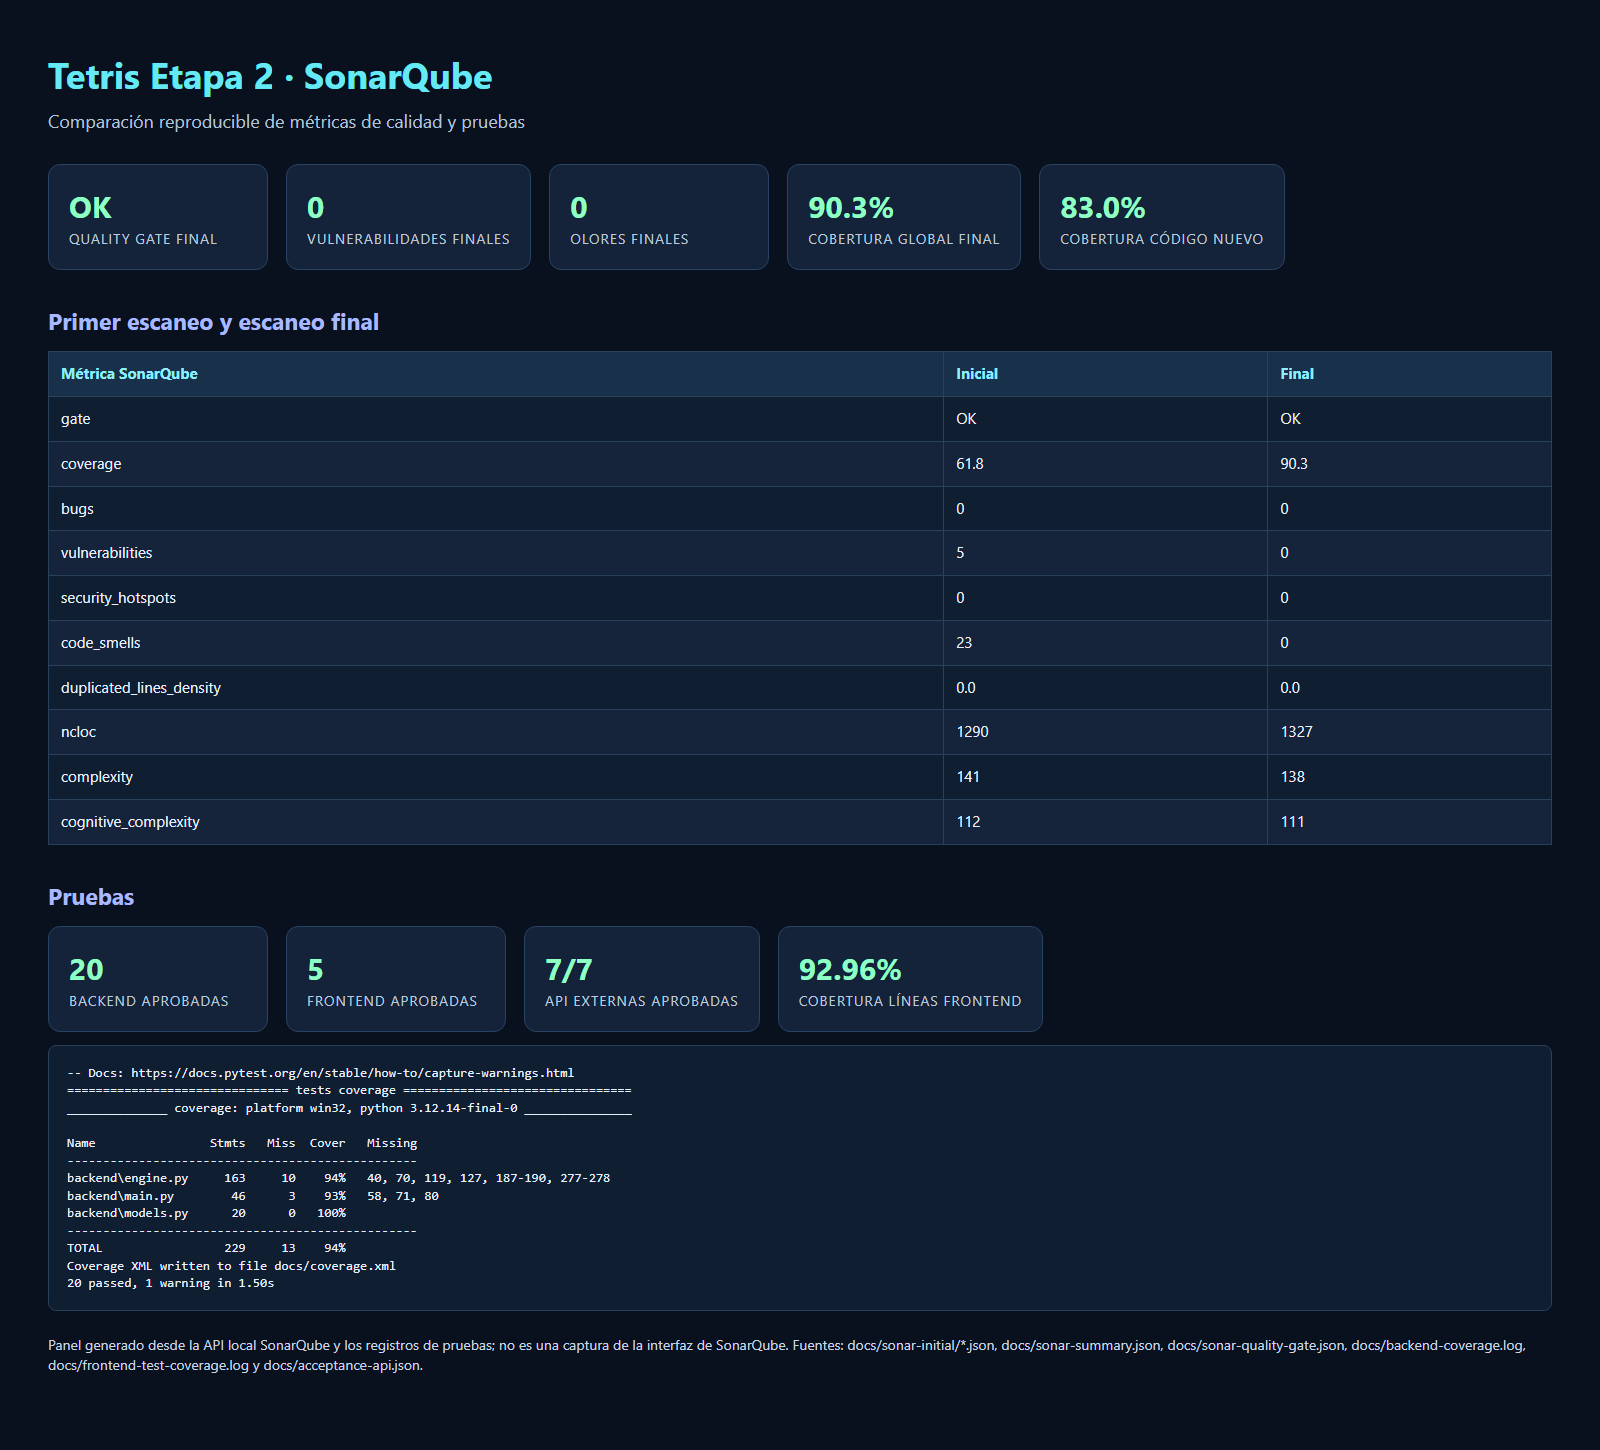
\includegraphics[width=.98\textwidth,height=.78\textheight,keepaspectratio]{tetris-etapa2-assets/openspec-sonar.png}
\caption{OpenSpec: panel elaborado por el investigador a partir de JSON de SonarQube y logs de pruebas. No es la interfaz web nativa de SonarQube.}\label{fig:openspec-sonar_tetris_e2}\end{figure}

\begin{figure}[H]\centering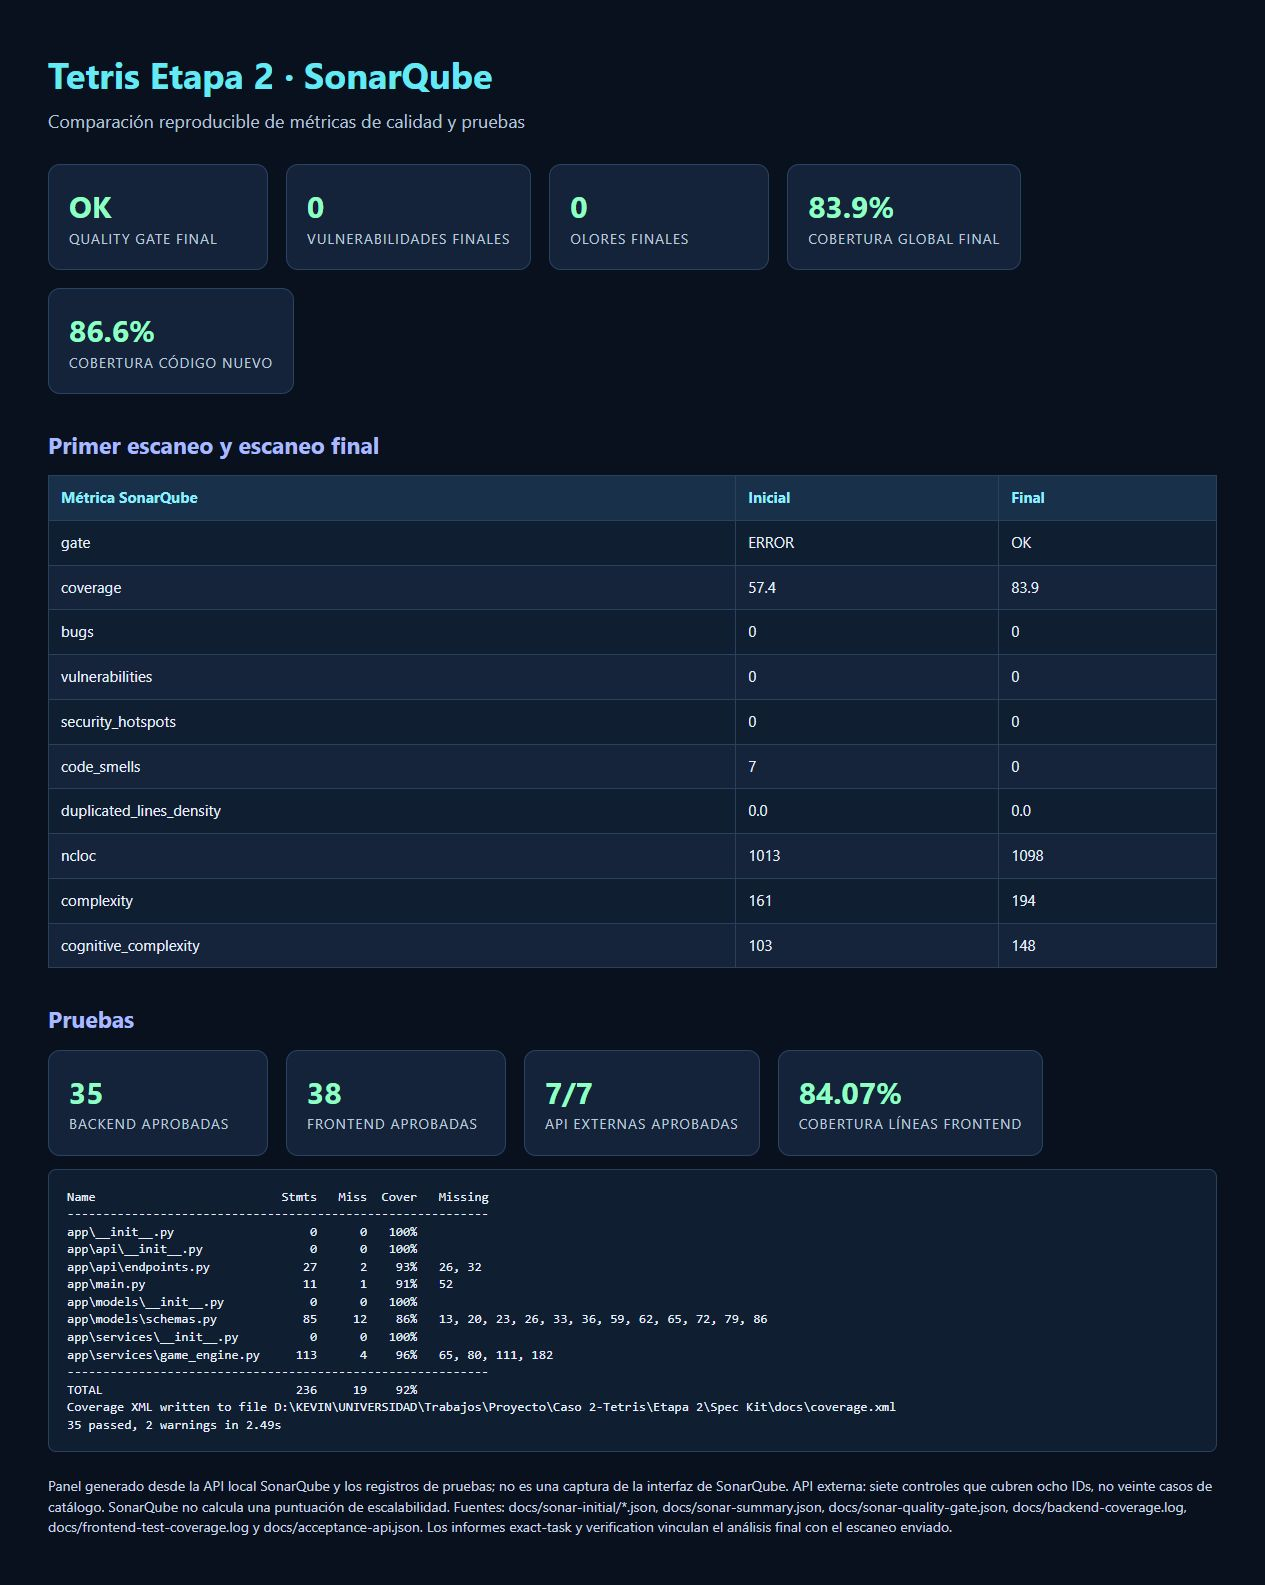
\includegraphics[width=.98\textwidth,height=.78\textheight,keepaspectratio]{tetris-etapa2-assets/speckit-sonar.jpg}
\caption{Spec Kit: panel del investigador con resultados de SonarQube. Los valores finales se contrastan con el análisis exacto y la tabla de condiciones.}\label{fig:speckit-sonar_tetris_e2}\end{figure}

\begin{figure}[H]\centering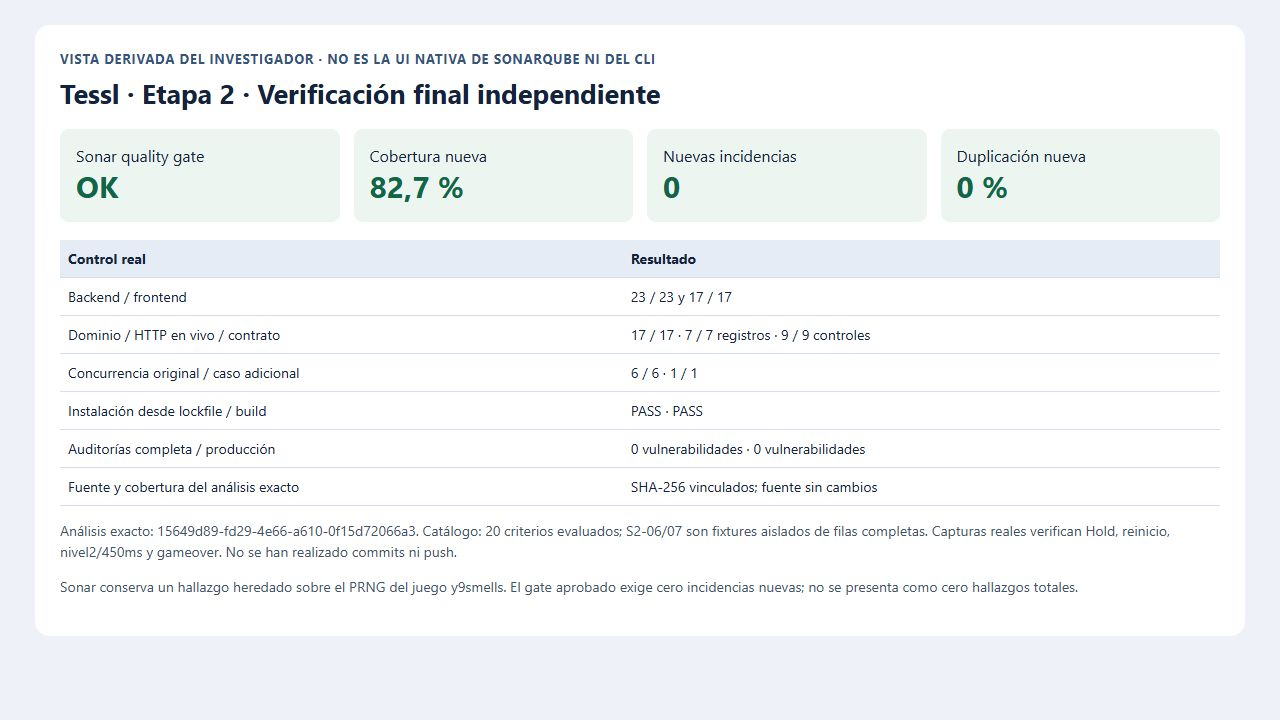
\includegraphics[width=.98\textwidth,height=.48\textheight,keepaspectratio]{tetris-etapa2-assets/tessl-sonar.jpg}
\caption{Tessl: vista del investigador derivada de la API de SonarQube, con hallazgos heredados separados del gate de código nuevo.}\label{fig:tessl-sonar_tetris_e2}\end{figure}

\begin{figure}[H]\centering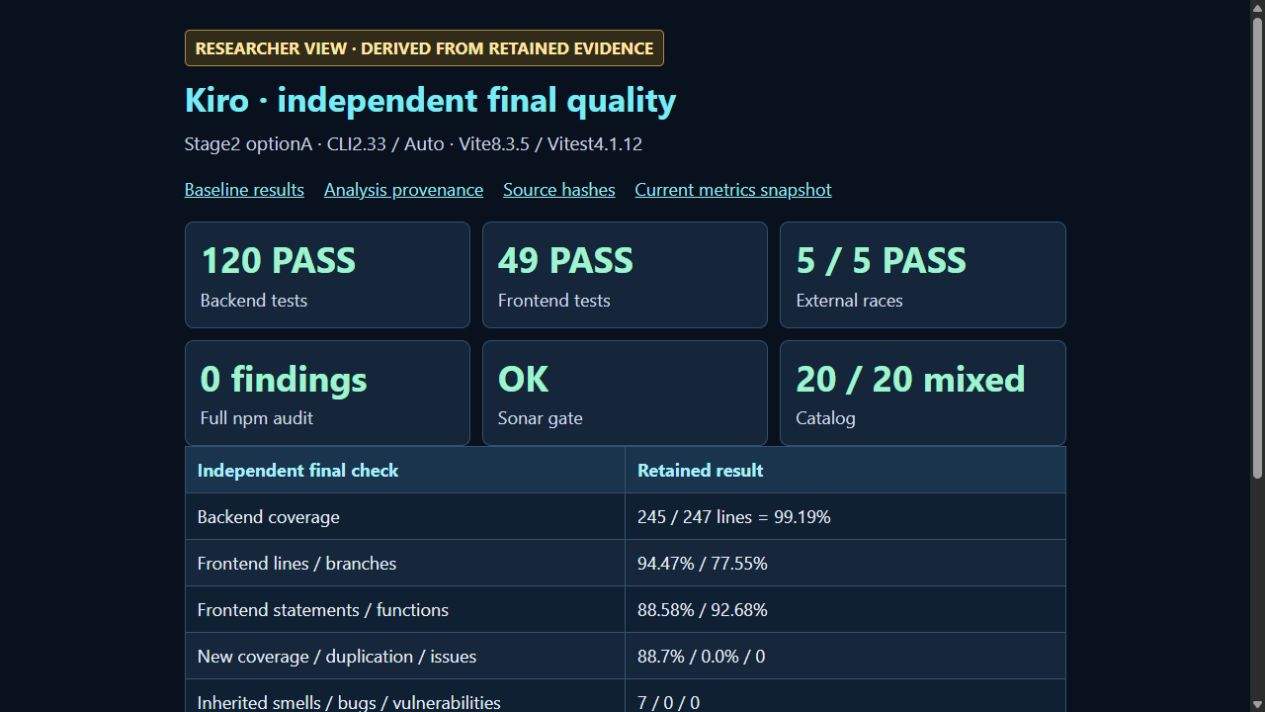
\includegraphics[width=.98\textwidth,height=.48\textheight,keepaspectratio]{tetris-etapa2-assets/kiro-sonar.jpg}
\caption{Kiro: panel del investigador derivado de SonarQube. No se atribuye a una captura de la interfaz nativa del producto.}\label{fig:kiro-sonar_tetris_e2}\end{figure}

\begin{figure}[H]\centering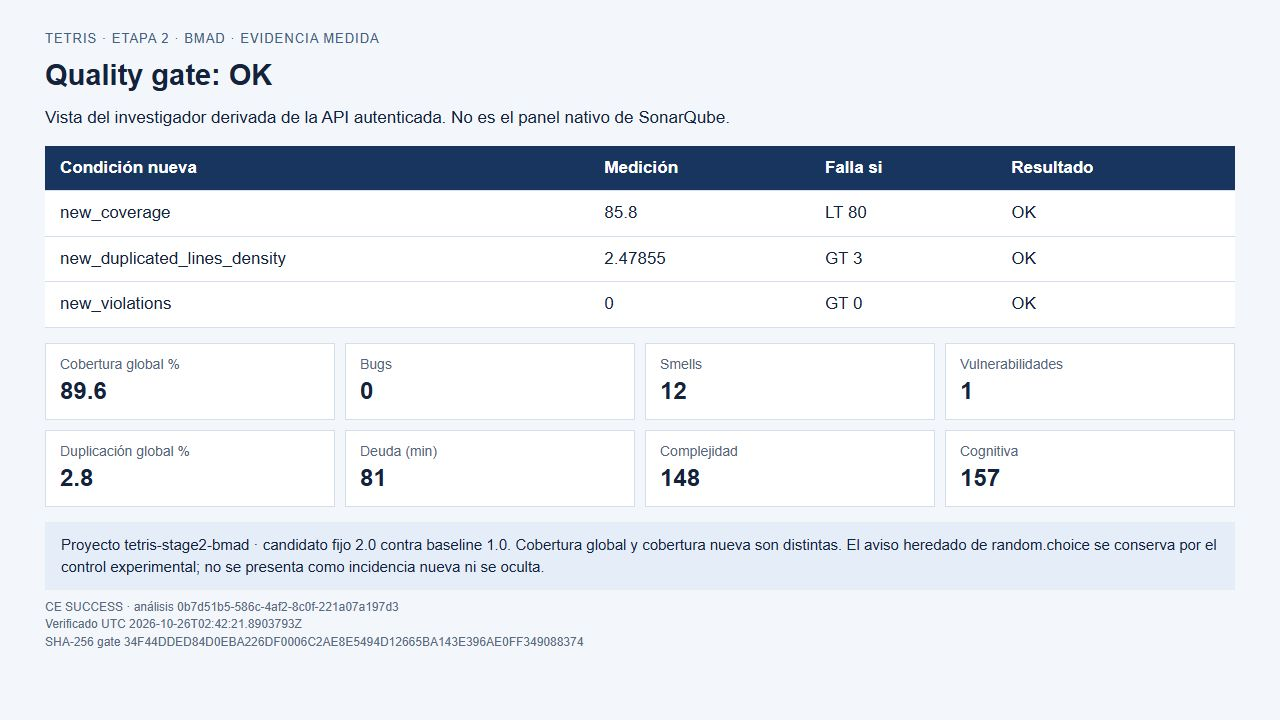
\includegraphics[width=.98\textwidth,height=.48\textheight,keepaspectratio]{tetris-etapa2-assets/bmad-sonar.jpg}
\caption{BMAD: panel del investigador del escaneo final, después de regenerar el XML de cobertura sobre la fuente congelada. Gate OK y cobertura global de 89,6~\%.}\label{fig:bmad-sonar_tetris_e2}\end{figure}

\begin{figure}[H]\centering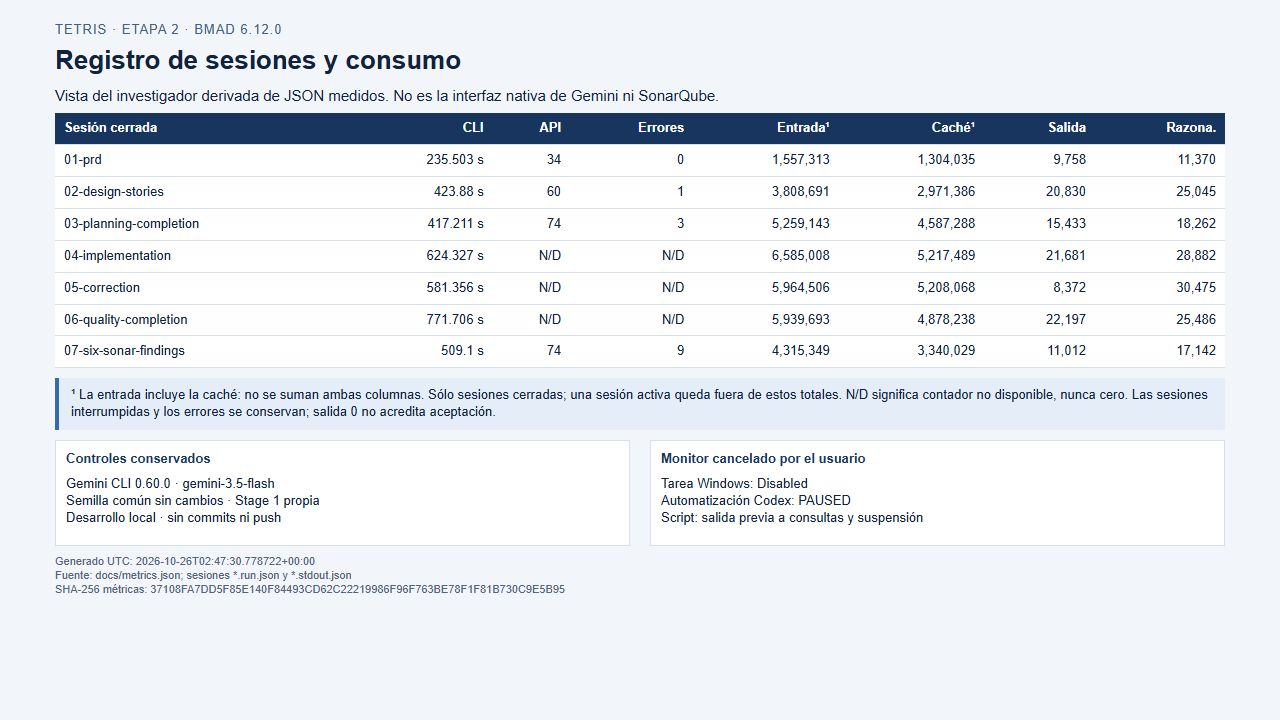
\includegraphics[width=.98\textwidth,height=.48\textheight,keepaspectratio]{tetris-etapa2-assets/bmad-uso.jpg}
\caption{BMAD: panel del investigador de las siete invocaciones, derivado de sus contadores originales. No es una pantalla nativa de facturación del proveedor.}\label{fig:bmad-uso_tetris_e2}\end{figure}

\paragraph{Trazabilidad por invocación.}

Las tablas siguientes conservan los valores de cada intento, incluidos los fallidos. ID corresponde al prefijo del nombre del registro \texttt{NN-*.run.json} bajo \texttt{docs/} de cada herramienta. I, C, O y P significan entrada, caché incluida, salida candidata y pensamiento; s es duración CLI. Se muestran tokens exactos, no aproximaciones en miles. N/D conserva vacíos del registro. Los indicadores de salida de proceso se resumen en las observaciones de la dimensión E; un resultado de proceso no reemplaza las pruebas de aceptación.

\begin{table}[H]\centering\small\setlength{\tabcolsep}{4pt}\renewcommand{\arraystretch}{1.06}
\caption{Registro por intento: OpenSpec}
\label{tab:sesiones_openspec_tetris_e2}
\begin{tabular*}{\textwidth}{@{\extracolsep{\fill}}l r r r r r}\toprule

\textbf{ID} & \textbf{s} & \textbf{I} & \textbf{C} & \textbf{O} & \textbf{P} \\ \midrule

01 & N/D & N/D & N/D & N/D & N/D \\

02 & 622,436 & 1.586.942 & 1.262.951 & 15.910 & 28.623 \\

03 & 137,359 & 2.141.393 & 1.591.392 & 6.694 & 7.116 \\

04 & 48,902 & 1.273.520 & 1.075.890 & 2.723 & 6.281 \\

05 & 444,118 & 2.623.509 & 2.252.478 & 4.391 & N/D \\

06 & 782,457 & 2.011.596 & 1.407.507 & 56.094 & 83.511 \\

07 & 167,938 & 382.138 & 197.261 & 6.667 & 12.209 \\

08 & 12,868 & 127.382 & 8.020 & 134 & 275 \\

09 & 237,026 & 541.005 & 253.683 & 8.066 & 15.663 \\

10 & 409,430 & 2.994.533 & 2.495.552 & 8.443 & 19.194 \\

\bottomrule\end{tabular*}

\end{table}

\begin{table}[H]\centering\small\setlength{\tabcolsep}{4pt}\renewcommand{\arraystretch}{1.06}
\caption{Registro por intento: Spec Kit}
\label{tab:sesiones_speckit_tetris_e2}
\begin{tabular*}{\textwidth}{@{\extracolsep{\fill}}l r r r r r}\toprule

\textbf{ID} & \textbf{s} & \textbf{I} & \textbf{C} & \textbf{O} & \textbf{P} \\ \midrule

01 & N/D & 372.306 & 328.077 & 572 & 3.622 \\

02 & 314,087 & 553.753 & 417.153 & 5.986 & 8.755 \\

03 & N/D & 231.106 & 152.515 & 5.847 & 18.651 \\

04 & 671,273 & 1.659.066 & 1.321.138 & 14.548 & 8.060 \\

05 & 304,671 & 293.607 & 155.479 & 4.874 & 6.352 \\

06 & 0,084 & 0 & 0 & 0 & 0 \\

07 & 545,391 & 1.065.684 & 505.891 & 8.216 & 7.163 \\

08 & 2.885,870 & 16.752.166 & 12.893.781 & 36.959 & 41.527 \\

09 & 3.450,181 & 10.900.997 & 8.551.042 & 40.048 & 42.080 \\

10 & 455,055 & 5.514.887 & 4.925.600 & 23.190 & 26.295 \\

11 & 439,318 & 607.848 & 257.143 & 2.297 & 16.381 \\

12 & 1.513,504 & 1.830.444 & 1.091.029 & 10.707 & 14.468 \\

13 & 16,638 & 225.989 & 104.499 & 144 & 630 \\

14 & 184,895 & 720.193 & 422.234 & 1.936 & 15.806 \\

15 & 56,315 & 160.759 & 0 & 1.808 & 7.575 \\

16 & 375,325 & 1.560.326 & 1.173.857 & 6.505 & 15.859 \\

17 & 313,986 & 1.540.447 & 1.116.692 & 4.735 & 8.890 \\

\bottomrule\end{tabular*}

\end{table}

\begin{table}[H]\centering\small\setlength{\tabcolsep}{4pt}\renewcommand{\arraystretch}{1.06}
\caption{Registro por intento: Tessl}
\label{tab:sesiones_tessl_tetris_e2}
\begin{tabular*}{\textwidth}{@{\extracolsep{\fill}}l r r r r r}\toprule

\textbf{ID} & \textbf{s} & \textbf{I} & \textbf{C} & \textbf{O} & \textbf{P} \\ \midrule

01 & 399,402 & 574.303 & 409.971 & 8.458 & 12.390 \\

02 & 5,813 & N/D & N/D & N/D & N/D \\

03 & 110,546 & 445.013 & 264.257 & 10.336 & 8.473 \\

04 & 187,086 & 319.343 & 142.817 & 11.582 & 14.592 \\

05 & 1.607,145 & 16.961.692 & 13.783.860 & 57.182 & 58.896 \\

06 & 193,479 & 859.933 & 464.197 & 3.850 & 6.770 \\

07 & 615,060 & 8.712.836 & 7.429.797 & 14.769 & 30.084 \\

08 & 523,706 & 11.831.655 & 9.608.584 & 14.548 & 18.398 \\

\bottomrule\end{tabular*}

\end{table}

\begin{table}[H]\centering\small\setlength{\tabcolsep}{4pt}\renewcommand{\arraystretch}{1.06}
\caption{Registro por intento: BMAD}
\label{tab:sesiones_bmad_tetris_e2}
\begin{tabular*}{\textwidth}{@{\extracolsep{\fill}}l r r r r r}\toprule

\textbf{ID} & \textbf{s} & \textbf{I} & \textbf{C} & \textbf{O} & \textbf{P} \\ \midrule

01 & 235,503 & 1.557.313 & 1.304.035 & 9.758 & 11.370 \\

02 & 423,880 & 3.808.691 & 2.971.386 & 20.830 & 25.045 \\

03 & 417,211 & 5.259.143 & 4.587.288 & 15.433 & 18.262 \\

04 & 624,327 & 6.585.008 & 5.217.489 & 21.681 & 28.882 \\

05 & 581,356 & 5.964.506 & 5.208.068 & 8.372 & 30.475 \\

06 & 771,706 & 5.939.693 & 4.878.238 & 22.197 & 25.486 \\

07 & 509,100 & 4.315.349 & 3.340.029 & 11.012 & 17.142 \\

\bottomrule\end{tabular*}

\end{table}

\begin{table}[H]\centering\small\setlength{\tabcolsep}{4pt}\renewcommand{\arraystretch}{1.06}
\caption{Registro por intento: Kiro, unidades nativas conocidas}
\label{tab:sesiones_kiro_tetris_e2}
\begin{tabularx}{\textwidth}{l Y Y Y}\toprule

\textbf{ID} & \textbf{Segundos CLI} & \textbf{Créditos} & \textbf{Observación} \\ \midrule

01 & 140,931 & N/D & Cuenta inicial; interrupción. \\

02 & 331,014 & 5,897180 & Nueva cuenta; Vibe observado. \\

03 & 395,730 & 8,026105 & Revisión nativa Spec. \\

04 & 1.796,250 & 49,458271 & Implementación inicial. \\

05 & N/D & N/D & Tramo retenido; cierre desconocido. \\

06 & 888,976 & 18,924292 & Reintento QA. \\

07 & 604,254 & 19,063515 & Corrección de cola/temporizador. \\

\bottomrule\end{tabularx}

\end{table}

\paragraph{Vinculación y límites del resultado.}

La identidad de cada escaneo permite distinguir el cierre final de sus resultados intermedios. El archivo complementario \path{tetris-etapa2-assets/tetris-etapa2-metricas.csv}, incluido en las fuentes de este documento, conserva los contadores por intento; sus celdas vacías son datos desconocidos, no ceros.

\begin{table}[H]\centering\small\setlength{\tabcolsep}{4pt}\renewcommand{\arraystretch}{1.06}
\caption{Identidad de los análisis finales con referencia exacta conservada}
\label{tab:identidad_tetris_e2}
\begin{tabularx}{\textwidth}{l Y}\toprule

\textbf{Herramienta} & \textbf{Identificador de análisis} \\ \midrule

Spec Kit & \path{acca3bf6-e8bc-4c46-8db4-932b8609326c} \\

Tessl & \path{15649d89-fd29-4e66-a610-0f15d72066a3} \\

BMAD & \path{0b7d51b5-586c-4af2-8c0f-221a07a197d3} \\

Kiro & \path{c9e3f4c9-35e0-4434-8dfd-3723413c0588} \\

OpenSpec & \path{1f1f136c-a5da-491d-bf6c-7fb28b3dc900} (estado CE SUCCESS en \path{sonar-task.json}). \\

\bottomrule\end{tabularx}

\end{table}

Los inventarios y los escaneos se contrastaron con \texttt{metrics.json}, \texttt{sonar-summary.json}, los JSON de condiciones del gate, las matrices de aceptación y los informes finales de cada herramienta. Los paquetes \texttt{final-verified/} y manifiestos de hashes vinculan fuentes, cobertura y evidencias cuando están disponibles; BMAD conserva un manifiesto final de 545 archivos. La bitácora enlazada al inicio mantiene el detalle cronológico, capturas adicionales y rutas de evidencia. Las imágenes de este caso son una selección explicada de ese registro, no la totalidad de sus capturas ni sustitutos de las pruebas.

Las cinco ampliaciones alcanzan los criterios comunes y el gate experimental final mediante mecanismos documentados; sus costes, tiempos y grados de intervención permanecen distintos y parcialmente observados. La lectura comparativa debe conservar la base heredada, la adaptación real de cada workflow, los contadores ausentes y las correcciones manuales o de evidencia declaradas. No se deriva un ganador causal, un coste facturado completo ni una garantía de escalabilidad a partir de estas ejecuciones.
